\if \kafli1

\begin{skilgr}{}
Ef $[a,b]$ er lokað bil í $\mathbb{R}$ og $x_{0},x_{1},\ldots,x_{n}$ eru rauntölur þannig að
$$
a = x_{0} < x_{1} < \cdots < x_{n-1} < x_{n} = b
$$
þá kallast mengið $S = \{x_{0},x_{1},\ldots,x_{n-1},x_{n}\}$ \textbf{skipting} (eða bútun) á bilinu $[a,b]$.

\vspace{2mm}

Bilin $[x_{i-1},x_{i}]$ fyrir $i \in \{1,\ldots,n\}$ nefnast \textbf{bútar} skiptingarinnar og talan $\Delta x_{i} = x_{i}-x_{i-1}$ nefnist \textbf{lengd} i-ta bútarins.

\vspace{2mm}

\noindent Stærðin $||S|| = \max\{\Delta x_{1},\ldots,\Delta x_{n}\}$ nefnist svo \textbf{norm} skiptingarinnar.
\end{skilgr}

\begin{ath}
Til upprifjunar þá er stærðin $\max\{\Delta x_{1},\ldots,\Delta x_{n}\}$ stærsta talan sem kemur fyrir í menginu.
\end{ath}

\begin{syn}{skiptingu bils}

Gefið er mengið $[0,1]$ og skiptingin $S = \left\{0,\frac{1}{3},\frac{1}{2},\frac{5}{6},1\right\}$. Tilgreinið alla búta skiptingarinnar, finnið lengd þeirra og tilreinum að lokum hvert norm skiptingarinnar er.

\vspace{2mm}

{\bf Lausn:} Bútar skiptingarinnar eru $\left[0,\frac{1}{3}\right]$, $\left[\frac{1}{3},\frac{1}{2}\right]$, $\left[\frac{1}{2},\frac{5}{6}\right]$ og $\left[\frac{5}{6},1\right]$ en lengdir þeirra eru
\setlength{\jot}{4mm}
\begin{align*}
\Delta x_{1} &= x_{1}-x_{0} = \frac{1}{3} - 0 = \frac{1}{3}, \;\;\; \Delta x_{2} = x_{2}-x_{1} = \frac{1}{2} - \frac{1}{3} = \frac{1}{6}\\ \Delta x_{3} &= x_{3}-x_{2} = \frac{5}{6} - \frac{1}{2} = \frac{1}{3} \; \text{ og } \; \Delta x_{4} = x_{4}-x_{3} = 1 - \frac{5}{6} = \frac{1}{6}
\end{align*}
Við sjáum því að norm skiptingarinnar er $||S|| = \frac{1}{3}$.

\begin{figure}[h]
\center
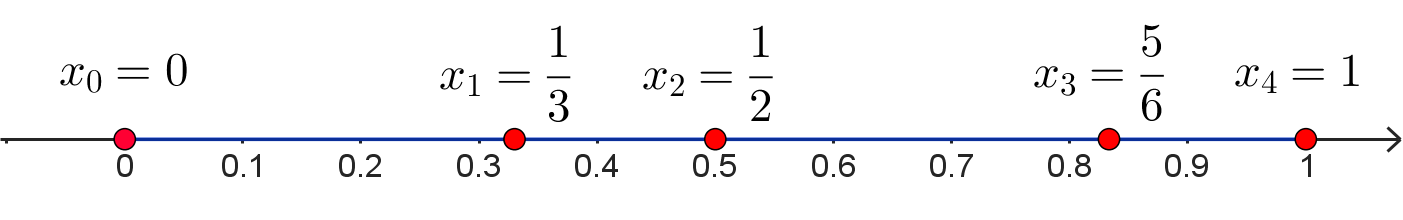
\includegraphics[width=0.95\textwidth]{Pictures/k2m1.png}
\caption{\it Myndræn framsetning á skiptingunni $S$ á bilinu $[0,1]$.}
\end{figure}

\end{syn}

\begin{skilgr}{}
Ef $S$ er skipting á bilinu $[a,b]$ og lengd allra búta $S$ er $\dfrac{b-a}{n}$ þar sem $n \in \mathbb{N}$ þá segjum við að $S$ sé \textbf{jöfn skipting} á bilinu $[a,b]$.
\end{skilgr}

\newpage

\begin{ath}
Ljóst er að jafna skiptingin í skilgreiningunni hér á undan hefur $n$ búta og að hún er ótvírætt ákvörðuð fyrir sérhvert bil $[a,b]$. Við munum hér eftir nota tákmálið $I_n$ til þess að tákna þessa skiptingu.
\end{ath}

\begin{syn}{jafna skiptingu}

Skrifum upp jöfnu skiptinguna með $3$ búta fyrir bilið $[0,1]$ og jöfnu skiptinguna með $5$ búta fyrir bilið $[0,2]$. Tilgreinum norm skiptinganna í hvoru tilfelli fyrir sig.

\vspace{2mm}

{\bf Lausn:} Ef við skiptum $[0,1]$ í $3$ búta með jafnri skiptingu þá er bútlengd hvers bútar $\frac{1-0}{3} = \frac{1}{3}$. Skiptingin er því $I_{3} = \left\{0,\frac{1}{3},\frac{2}{3},1\right\}$. Ef við skiptum svo bilinu $[0,2]$ upp í $5$ búta með jafnri skiptingu þá er bútlengd hvers bútar $\frac{2-0}{5} = \frac{2}{5}$. Skiptingin er þar með $I_{5} = \left\{0,\frac{2}{5},\frac{4}{5},\frac{6}{5},\frac{8}{5},2\right\}$.

\end{syn}

\begin{skilgr}{}
Ef $S$ og $T$ eru tvær skiptingar á bilinu $[a,b]$ og $S \subseteq T$ þá er $S$ sögð \textbf{grófari} en $T$. $T$ er einnig sögð vera \textbf{fínni} en $S$.
\end{skilgr}

\begin{ath}
Skilgreiningin hér að ofan segir einfaldlega að ef við byjum með einhverja skiptingu $S$ á bilinu $[a,b]$ og bætum svo fleiri skiptipunktum við hana þá fæst skipting sem er fínni en sú sem byrjað var með.
\end{ath}

\begin{skilgr}{}
Gefið er fall $f$ á $[a,b]$ og skipting $S = \{x_{0},\ldots,x_{n}\}$. 
\begin{itemize}

\item[1)] Ef til eru tölur $k_{1},\ldots,k_{n}$ þannig að
$$
k_{i} \leq f(x) \; \text{ fyrir öll } \; x \in [x_{i-1},x_{i}]
$$
þá kallast summan
$$
U_{S} = \sum_{i = 1}^{n} k_{i}\Delta x_{i}
$$
\textbf{undirsumma} fyrir fallið $f$ á bilinu $[a,b]$ með tilliti til skiptingarinnar $S$.

\end{itemize}
\end{skilgr}

\newpage

\begin{bluebox}{}
\begin{itemize}

\item[2)] Ef til eru tölur $K_{1},\ldots,K_{n}$ þannig að
$$
f(x) \leq K_{i} \; \text{ fyrir öll } \; x \in [x_{i-1},x_{i}]
$$
þá kallast summan
$$
Y_{S} = \sum_{i = 1}^{n} K_{i}\Delta x_{i}
$$
\textbf{yfirsumma} fyrir fallið $f$ á bilinu $[a,b]$ með tilliti til skiptingarinnar $S$.

\item[3)] Ef við veljum tölur $t_{i} \in [x_{i-1},x_{i}]$ fyrir öll $i \in \{1,\ldots,n\}$ þá kallast summan
$$
\sigma_{S} = \sum_{i = 1}^{n} f\left(t_{i}\right)\Delta x_{i}
$$
\textbf{millisumma} (eða Riemann summa) fyrir fallið $f$ á bilinu $[a,b]$ með tilliti til skiptingarinnar $S$.

\end{itemize}
\end{bluebox}

\begin{ath}
Út frá skilgreiningunni er ljóst að fyrir sérhverja skiptingu $S$ á bili $[a,b]$ og fall $f$ skilgreint á því bili gildir að
$$
U_{S} \leq \sigma_{S} \leq Y_{S}
$$
\end{ath}

\begin{ath}
Í skilgreiningunni hér að ofan var nóg að velja $k_i$ sem einhverja tölu þannig að $k_i \leq f(x)$ fyrir öll $x \in [x_{i-1},x_{i}]$. Nema annað sé tekið fram þá munum við alltaf ganga út frá að $k_i$ hafi verið valið sem \textbf{lággildi} $f$ á bilinu $[x_{i-1},x_{i}]$. Vert er að nefna að til eru föll sem hafa ekki endilega lággildi á lokuðu bili, en við munum ekki skoða slík föll í þessu hefti. Eins munum við ætíð ganga út frá að $K_i$ hafi verið valið sem \textbf{hágildi} fallisin $f$ á bilinu $[x_{i-1},x_{i}]$. Að endingu munum við svo alltaf velja $t_{i}$ sem miðpunkt bilsins $[x_{i-1},x_{i}]$, þ.e.
$$
t_{i} = \frac{x_{i-1}+x_{i}}{2}
$$
\end{ath}

\begin{ath}
Óformlega er hægt er að líta á sérhvern lið í summunum sem flatarmál ákveðins ferhyrnings. Ferhyrningarnir sem um ræðir í tilfelli undirsummunar eru þeir ferhyrningar sem hafa búta skiptingarinnar sem grunnlínu, en hæð þeirra er síðan lægsta gildi fallsins $f$ á hverjum bút.  Fyrir yfir- og millisummuna er um sömu grunnlínur að ræða, en hæðirnar eru hæstu gildi $f$ í tilfelli yfirsummunar, en fallgildi $f$ í miðpunktum bútanna í tilfelli millisummunar.

\newpage

\begin{figure}[H]
\center
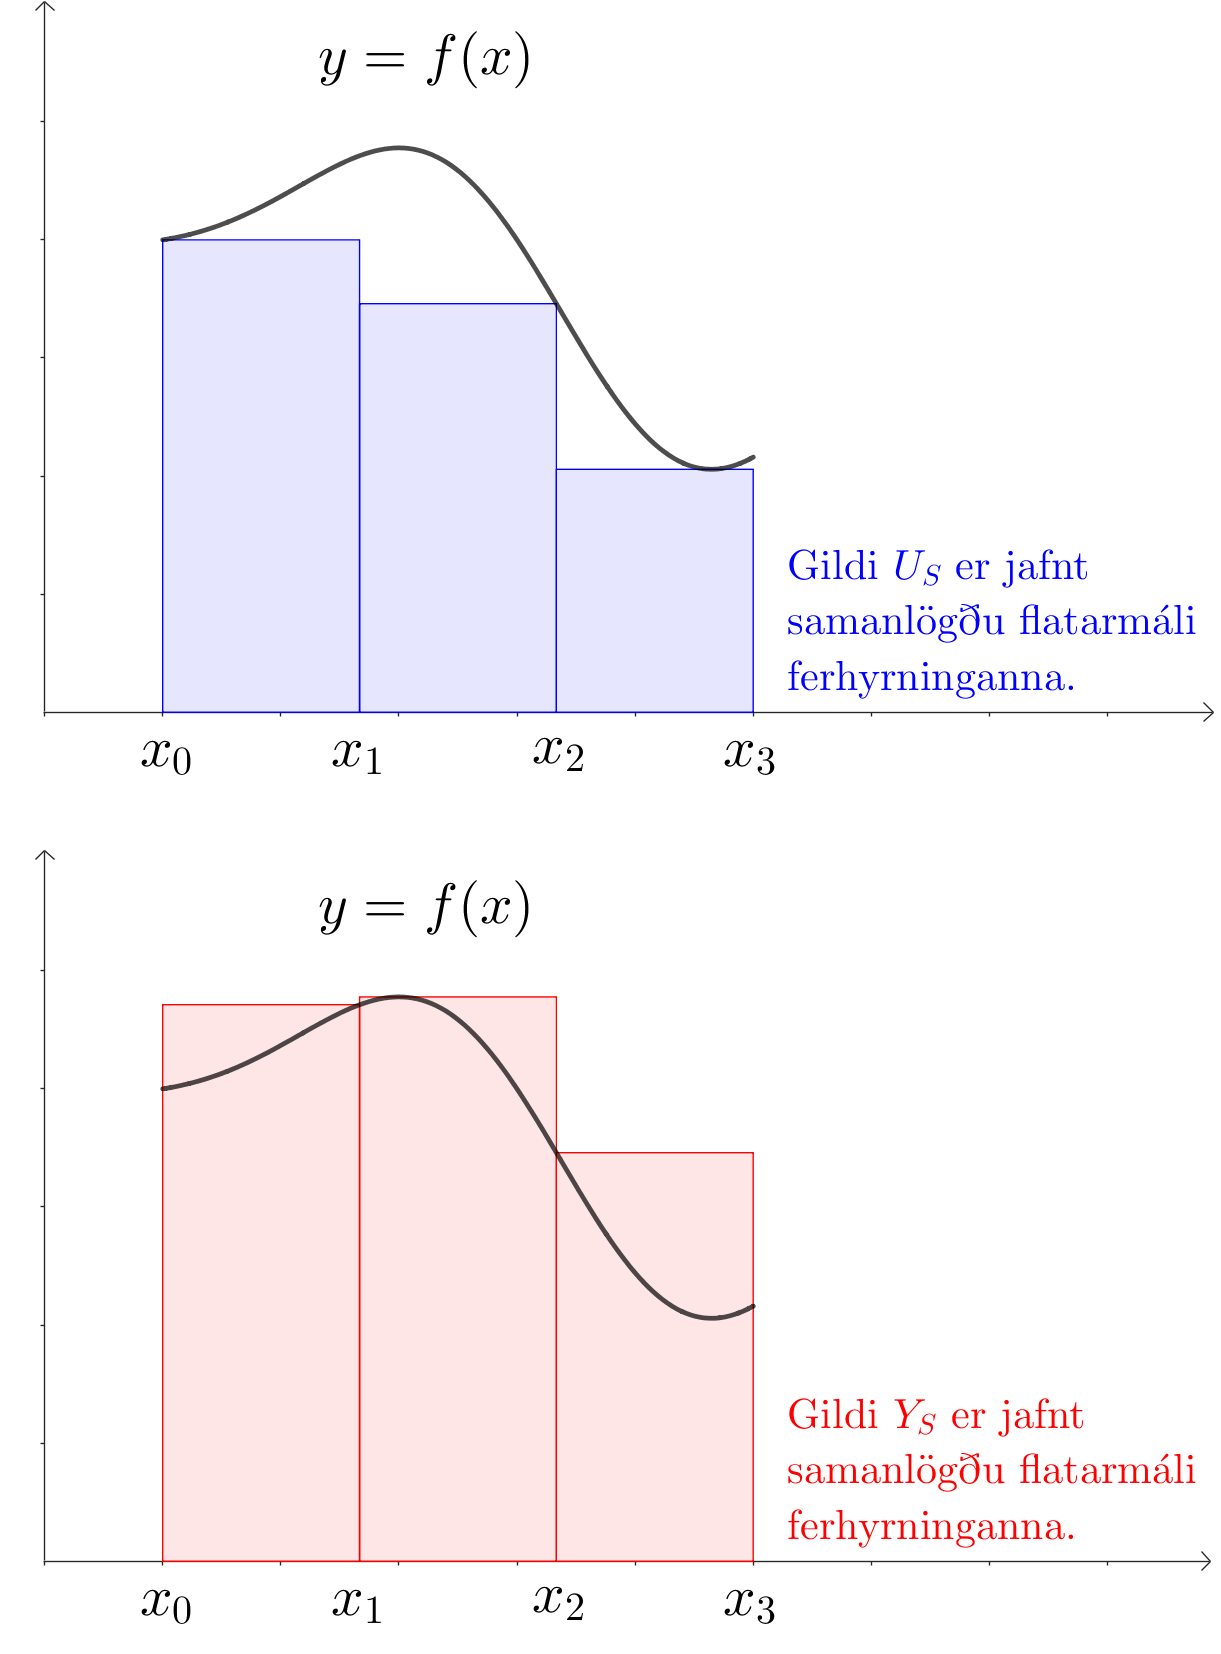
\includegraphics[width=0.95\textwidth]{Pictures/k2m6.png}
\caption{\it Myndræn framsetning á undir- og yfirsummu falls $f$ með skiptinguna $S = \{x_{0},x_{1},x_{2},x_{3}\}$ á bilinu $[a,b]$.}
\end{figure}

\newpage

\begin{figure}[H]
\center
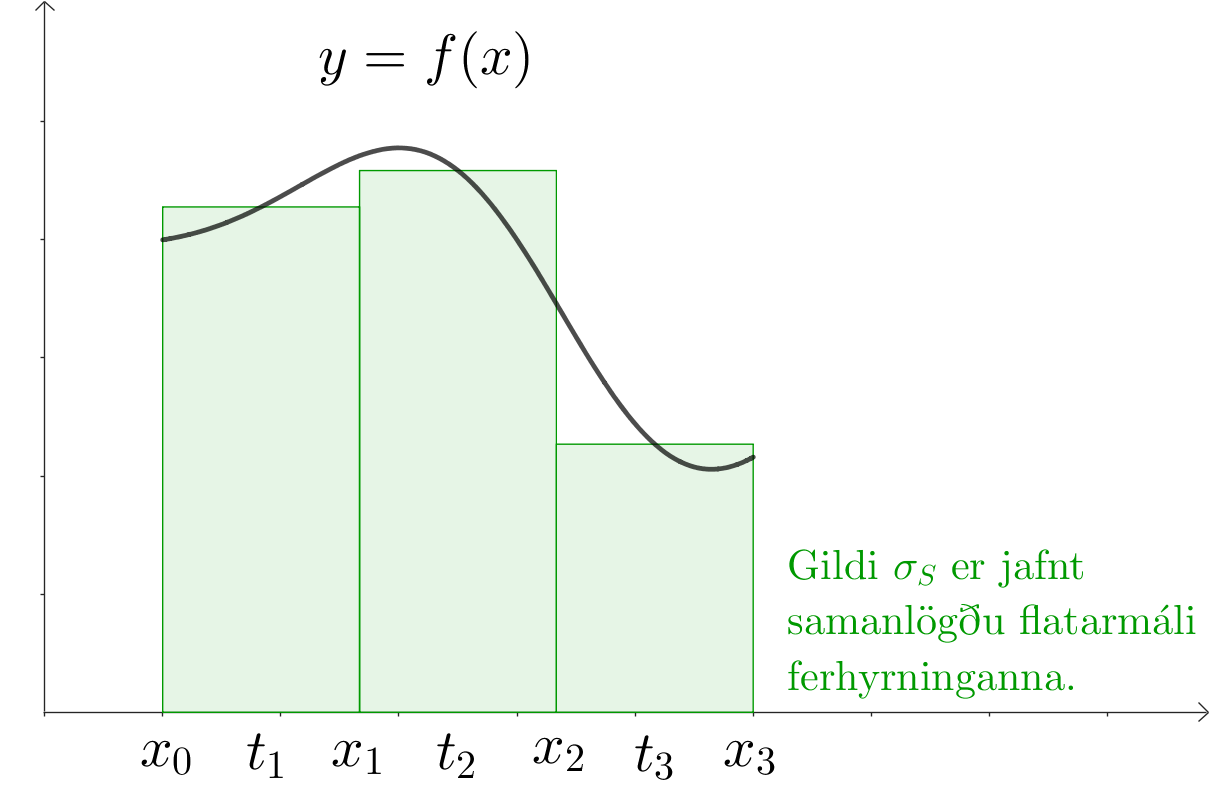
\includegraphics[width=0.95\textwidth]{Pictures/k2m7.png}
\caption{\it Myndræn framsetning á millisummu falls $f$ með skiptinguna $S = \{x_{0},x_{1},x_{2},x_{3}\}$ á bilinu $[a,b]$.}
\end{figure}
\end{ath}

\begin{ath}
Ef $S$ er skipting á bili $[a,b]$ og við viljum finna há- og lágildi falls $f$ á öllum bútum skiptingarinnar þá þurfum við að gera formerkjamynd fyrir afleiðu $f$ og finna útgildi fallsins á öllum bútum skiptingarinnar. Það er þó ekki nauðsynlegt í öllum tilfellum, t.d. þegar fallið $f$ er \textbf{einhalla}. Þannig fæst að ef $f$ er \textbf{vaxandi} á bilinu þá mun það taka lágildi í vinstri endapunkti sérhvers bútar, en hágildi í hægri endapunktinum. Ef $f$ er svo \textbf{minnkandi} á bilinu þá mun það taka hágildi í vinstri endapunkti sérhvers bútar, en lágildi í hægri endapunktinum.
\end{ath}

\begin{syn}{undir- yfir- og millisummur}
Gefið er fallið $f(x) = x^{2}$ á bilinu $[0,2]$ og jafna skiptingin $I_4 = \left\{0,\frac{1}{2},1,\frac{3}{2},2\right\}$. Reiknið undir-, yfir- og millisummur fallsins $f$ m.t.t. skiptingarinnar.

\vspace{2mm}

{\bf Lausn} Þar sem fallið $f$ er vaxandi á $[0,2]$ þá tekur það lægstu gildi sýn í vinstri endapunkti sérhvers bútar, en hæstu gildi sýn í hægri endapunkti sérhvers bútar. Athugum einnig að bútlengd sérhvers bútar er $\frac{1}{2}$. Við fáum því að
\setlength{\jot}{4mm}
\begin{align*}
U_{I_{4}} &= f(0)\cdot\frac{1}{2}+f\left(\frac{1}{2}\right)\cdot\frac{1}{2}+f(1)\cdot\frac{1}{2}+f\left(\frac{3}{2}\right)\cdot\frac{1}{2}\\ &= \frac{1}{2}\cdot\left(0^{2}+\left(\frac{1}{2}\right)^{2}+1^{2}+\left(\frac{3}{2}\right)^{2}\right) = 1.75
\end{align*}

\begin{figure}[H]
\center
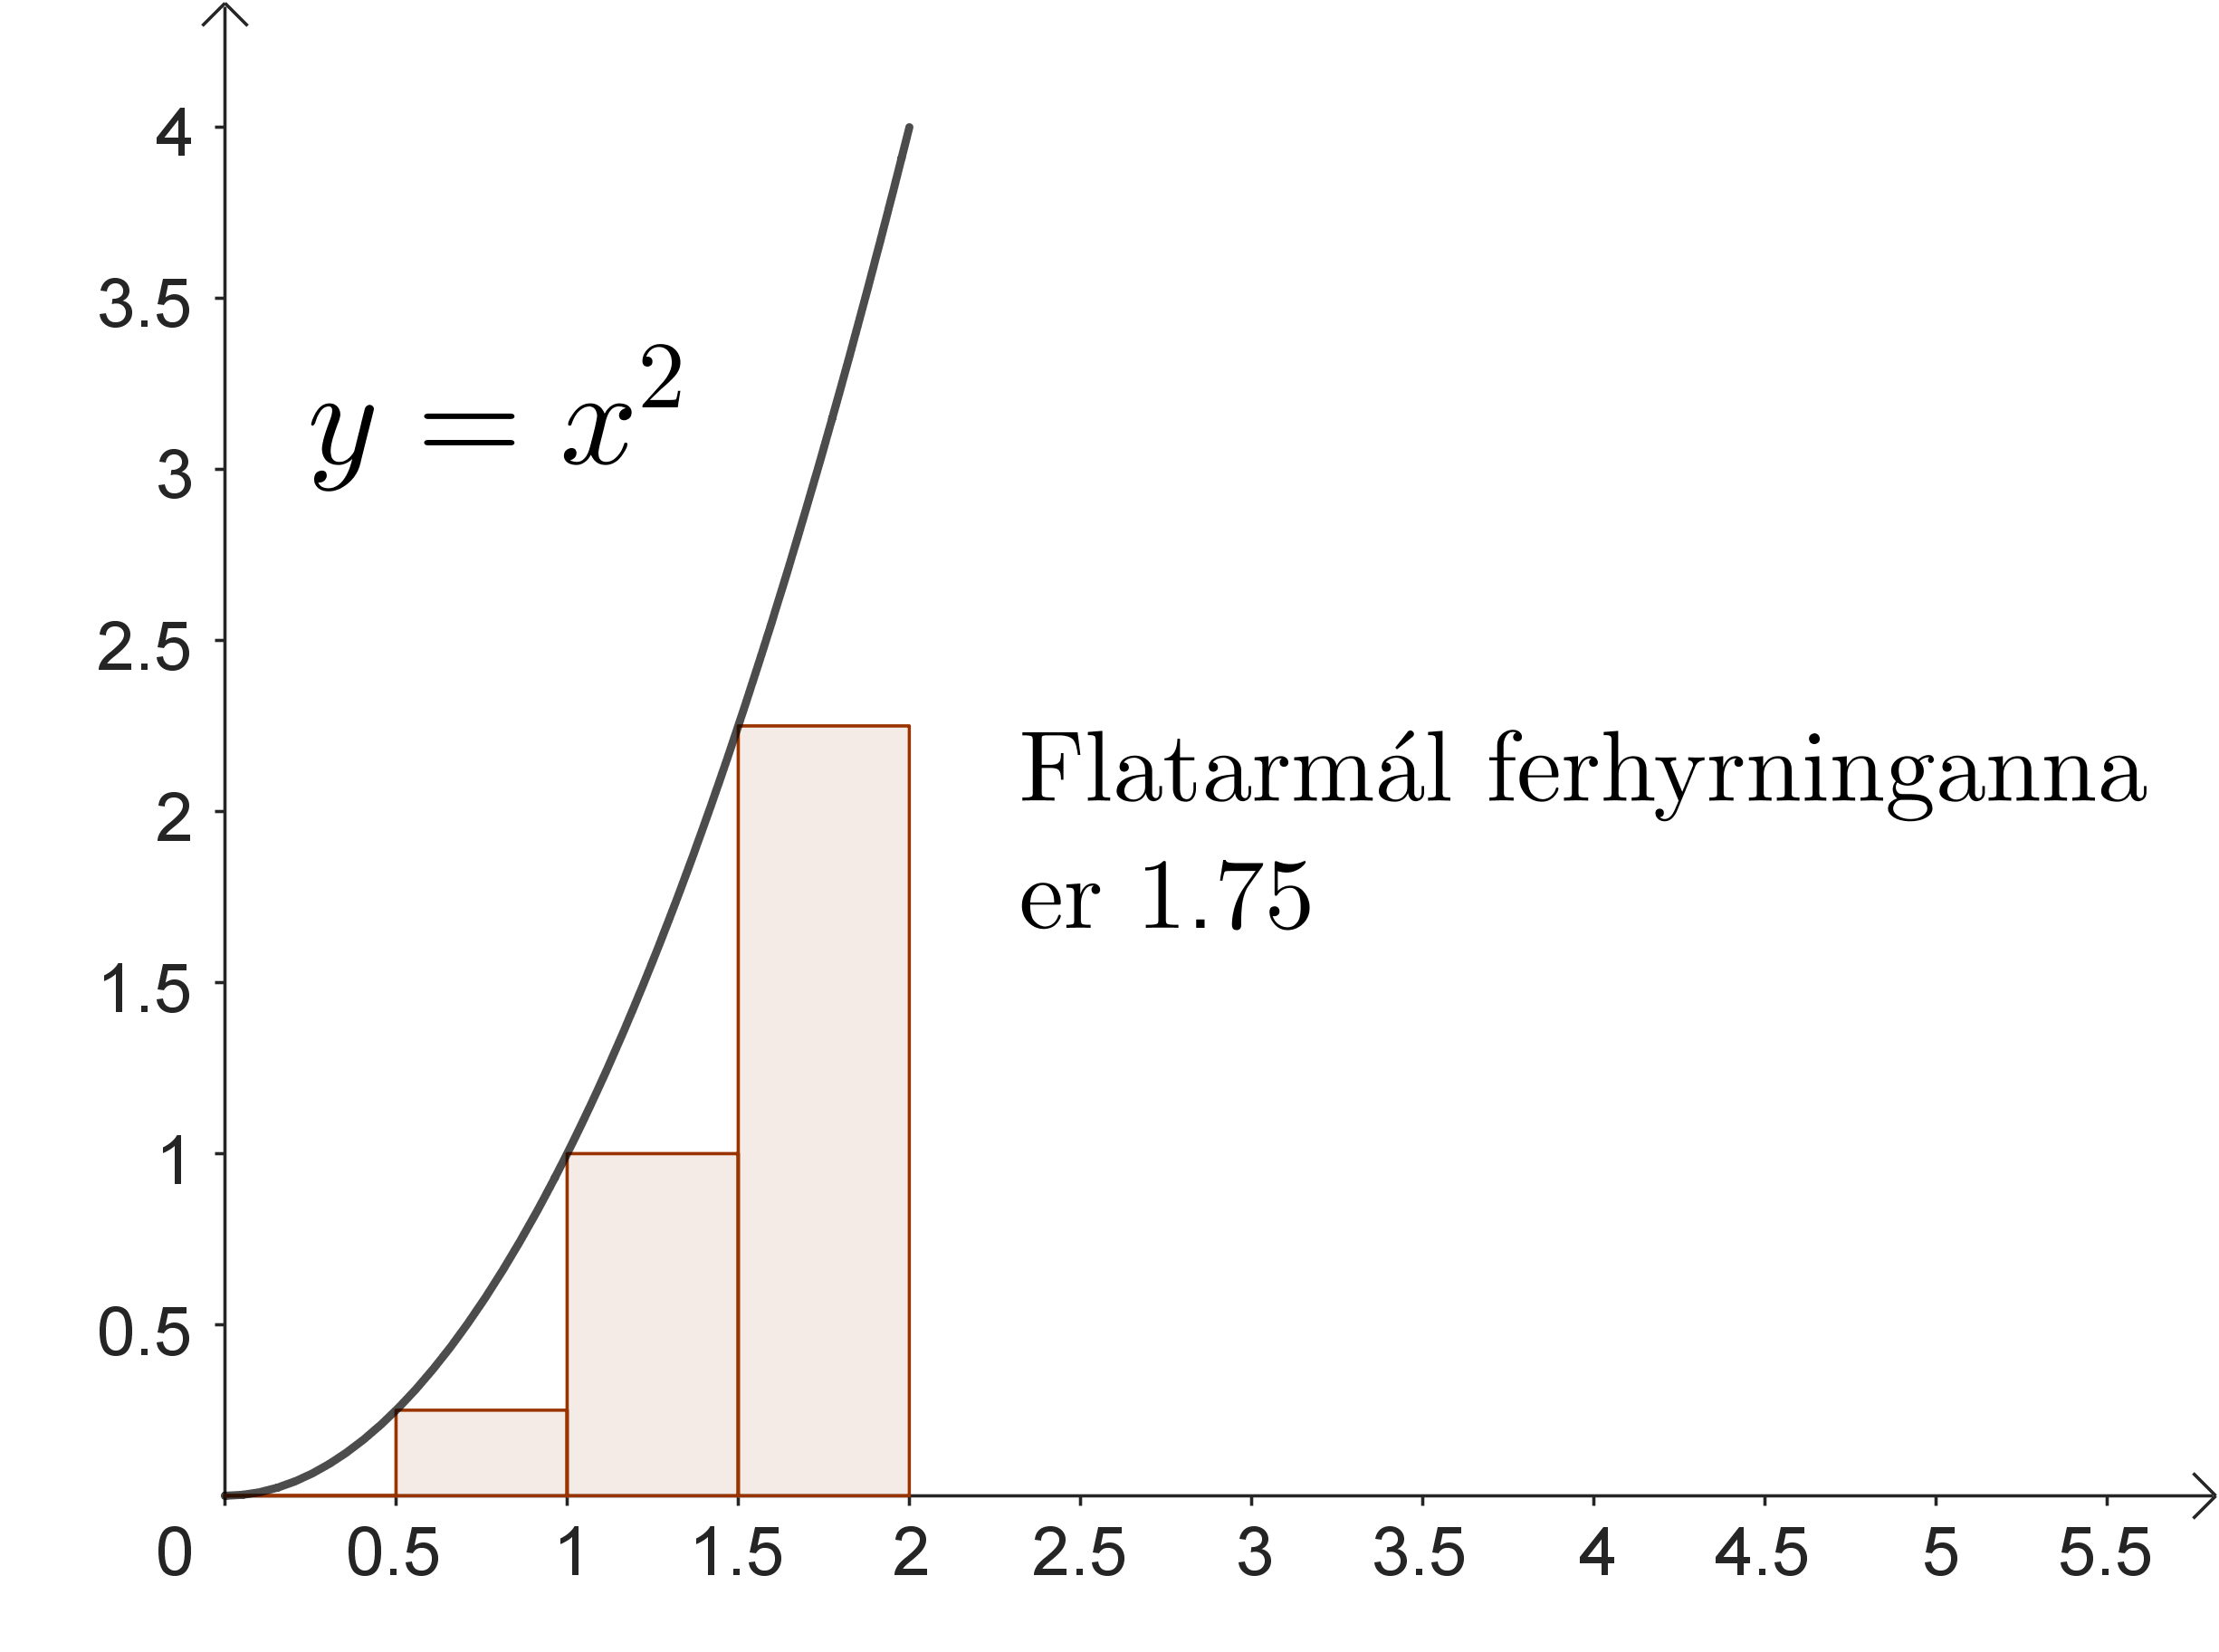
\includegraphics[width=0.8\textwidth]{Pictures/k2m2.png}
\caption{\it Myndræn framsetning á undursummu $f$ m.t.t. skiptingarinnar $I_4$.}
\end{figure}

Eins fæst að yfirsumman er

\begin{align*}
Y_{I_{4}} &= f\left(\frac{1}{2}\right)\cdot\frac{1}{2}+f\left(1\right)\cdot\frac{1}{2}+f\left(\frac{3}{2}\right)\cdot\frac{1}{2}+f\left(2\right)\cdot\frac{1}{2}\\ &= \frac{1}{2}\cdot\left(\left(\frac{1}{2}\right)^{2}+1^{2}+\left(\frac{3}{2}\right)^{2}+2^{2}\right) = 3.75
\end{align*}

\vspace{2mm}

Við sjáum svo að miðpunktar bútanna eru $t_{1} = \frac{1}{4}$, $t_{2} = \frac{3}{4}$, $t_{3} = \frac{5}{4}$ og $t_{4} = \frac{7}{4}$. Millisumman er því
\begin{align*}
\sigma_{I_{4}} &= f\left(\frac{1}{4}\right)\cdot\frac{1}{2}+f\left(\frac{3}{4}\right)\cdot\frac{1}{2}+f\left(\frac{5}{4}\right)\cdot\frac{1}{2}+f\left(\frac{7}{4}\right)\cdot\frac{1}{2}\\ &= \frac{1}{2}\cdot\left(\left(\frac{1}{4}\right)^{2}+\left(\frac{3}{4}\right)^{2}+\left(\frac{5}{4}\right)^{2}+\left(\frac{7}{4}\right)^{2}\right) = 2.625
\end{align*}

\newpage

\begin{figure}[H]
\center
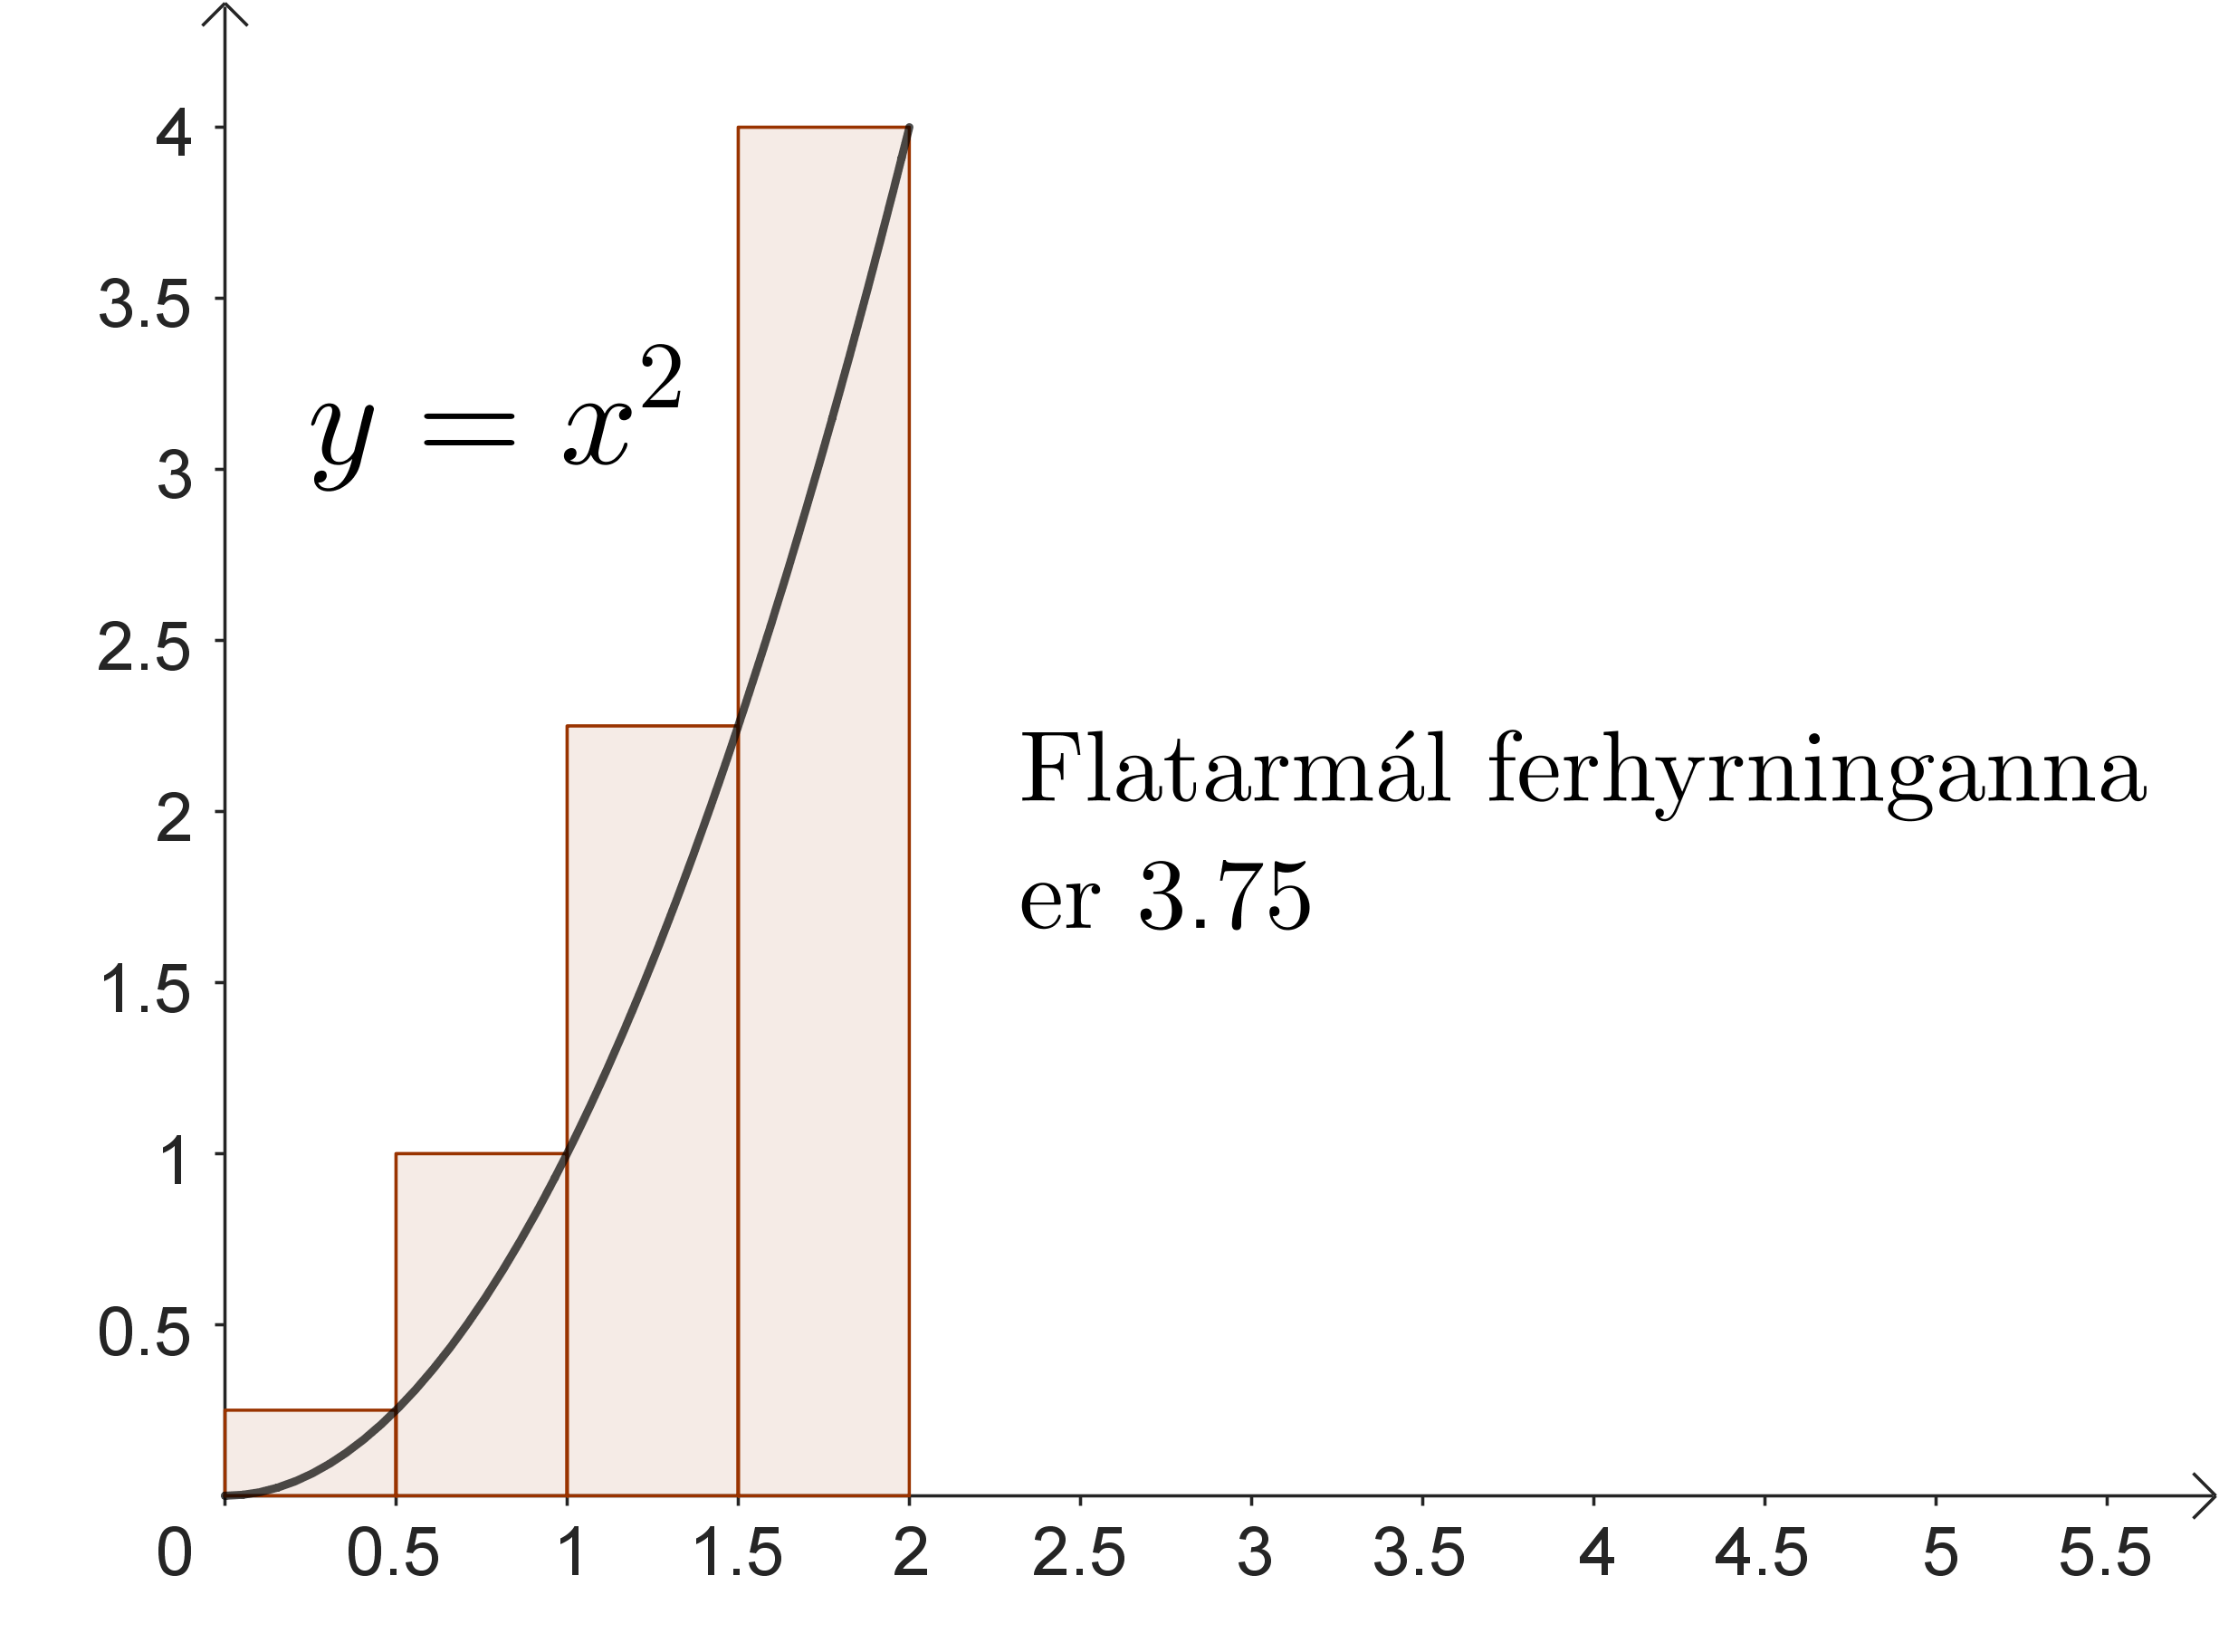
\includegraphics[width=0.8\textwidth]{Pictures/k2m3.png}
\caption{\it Myndræn framsetning á yfirsummu $f$ m.t.t. skiptingarinnar $I_4$.}
\end{figure}

\begin{figure}[H]
\center
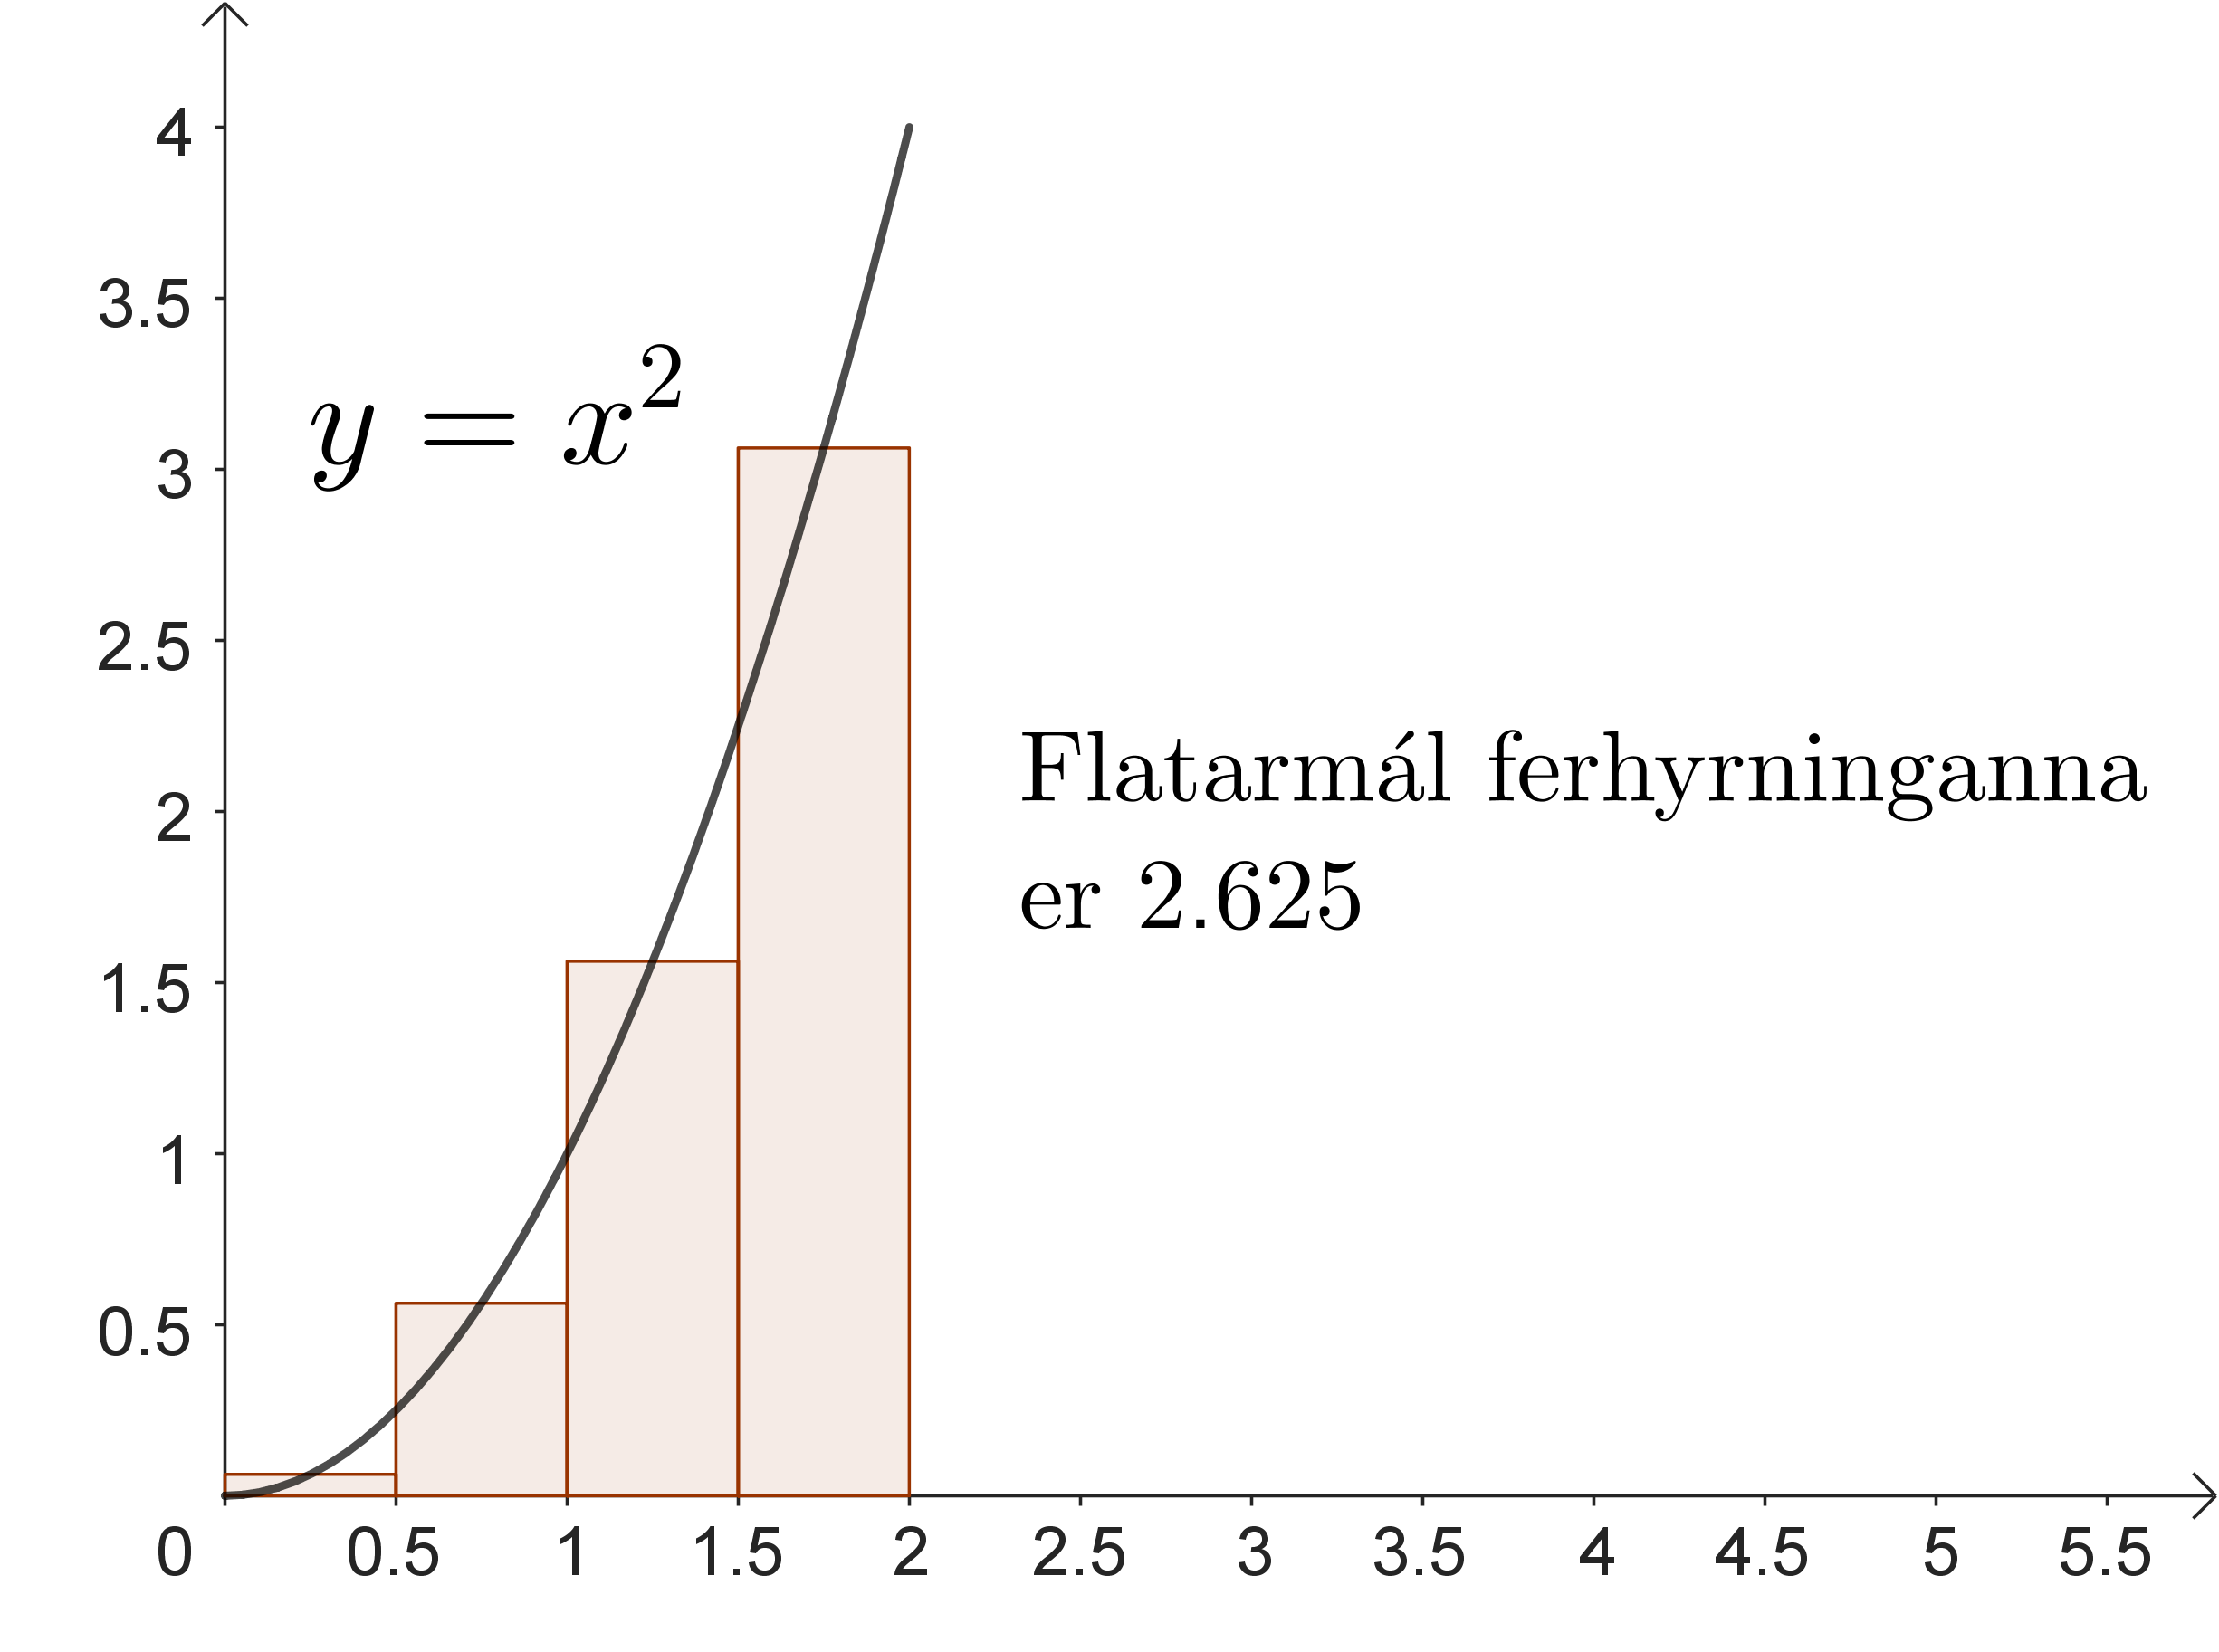
\includegraphics[width=0.8\textwidth]{Pictures/k2m4.png}
\caption{\it Myndræn framsetning á millisummu $f$ m.t.t. skiptingarinnar $I_4$.}
\end{figure}

\end{syn}

\begin{syn}{undir- yfir- og millisummur}
Gefið er fallið $f(x) = \frac{1}{x}$ á bilinu $[1,2]$ og skiptingin $S = \left\{1,\frac{4}{3},\frac{3}{2},2\right\}$. Reiknið undir-, yfir- og millisummur fallsins $f$ m.t.t. skiptingarinnar.

\vspace{2mm}

{\bf Lausn:} Athugum að fallið $f(x) = \frac{1}{x}$ er minnkandi á bilinu $[1,2]$. Þar með tekur það lággildi í hægri endapunktum sérhvers bútar, en hágildi í þeim vinstri. Við fáum þar með
\setlength{\jot}{4mm}
\begin{align*}
U_{S} &= f\left(\frac{4}{3}\right)\cdot \Delta x_{1} + f\left(\frac{3}{2}\right)\cdot\Delta x_{2} + f\left(2\right)\cdot \Delta x_{3}\\ &= \frac{3}{4}\cdot\frac{1}{3} + \frac{2}{3}\cdot\frac{1}{6} + \frac{1}{2}\cdot\frac{1}{2} = \frac{11}{18} = 0.611
\end{align*}
og eins
\begin{align*}
Y_{S} &= f\left(1\right)\cdot \Delta x_{1} + f\left(\frac{4}{3}\right)\cdot\Delta x_{2} + f\left(\frac{3}{2}\right)\cdot \Delta x_{3}\\ &= 1\cdot\frac{1}{3}+\frac{3}{4}\cdot\frac{1}{6}+\frac{2}{3}\cdot\frac{1}{2} = \frac{19}{24} = 0.792
\end{align*}
Við sjáum svo að miðpunktar bútanna eru $t_{1} = \frac{7}{6}$, $t_{2} = \frac{17}{12}$ og $t_{3} = \frac{7}{4}$. Millisumman er því
\begin{align*}
\sigma_{S} &= f\left(\frac{7}{6}\right)\cdot\Delta x_{1} + f\left(\frac{17}{12}\right)\cdot\Delta x_{2} + f\left(\frac{7}{4}\right)\cdot\Delta x_{3}\\
&= \frac{6}{7}\cdot\frac{1}{3}+\frac{12}{17}\cdot\frac{1}{6}+\frac{4}{7}\cdot\frac{1}{2} = \frac{82}{119} = 0.689
\end{align*}

\end{syn}

\begin{syn}{undir- og yfirsummur}
Gefið er fallið $f(x) = x^3-2x^2+1$ á bilinu $\left[-\frac{1}{2},2\right]$. Gerið formerkjamynd fyrir afleiðu $f$ og notið hana svo til þess að reikna undir- og yfirsummu fallsins á bilinu m.t.t. skiptingarinnar $S =\left\{-\frac{1}{2},\frac{1}{2},1,2\right\}$.

\vspace{2mm}

{\bf Lausn:} Byrjum á að diffra $f$, fáum $f'(x) = 3x^{2}-4x = x\left(3x-4\right)$. Sjáum því að $f'(x) = 0$ ef $x = 0$ eða $x = \frac{4}{3}$. Prófun gefur svo að $f'(x) < 0$ ef $x \in \left]0,\frac{4}{3}\right[$ en $f'(x) > 0$ ef $x \in \left[-\frac{1}{2},0\right[ \cup \left]\frac{4}{3},2\right]$. 

\begin{center}
\scalebox{1.3}
{
\begin{tikzpicture}[mynd, x=1.0cm, y=1.0cm]
\draw[asar] (-1.5,0) -- (3,0)
node[formerki_staerd] {$f'(x)$}
node[rot, anchor=south, shift={(0,4pt)}] (linan) {$x$} ;
\foreach \x in {0,1.33}
\draw[xkvardi, shift={(\x,0)}] (0pt,-3pt) -- (0pt,3pt) node[rot] {$\x$};
    \draw  (-0.75,0)  node[formerki] {$+$};
    \draw  (0,0)   node[formerki] {$0$};
    \draw (0.67,0) node[formerki] {$-$};
    \draw (1.33,0) node[formerki] {$0$};
    \draw (2.15,0) node[formerki] {$+$};
\end{tikzpicture}
}
\end{center}

Við getum nú notast við formerkjamyndina hér að ofan til þess að reikna undir- og yfirsummur $f$ m.t.t $S$. Byrjum á undirsummunni. 

\vspace{2mm}

Á bútnum $\left[-\frac{1}{2},\frac{1}{2}\right]$ tekur $f$ lágildi í öðrum hvorum endapunktinum. Við höfum að $f\left(-\frac{1}{2}\right) = \frac{3}{8}$ en $f\left(\frac{1}{2}\right) = \frac{5}{8}$ svo $f$ hefur þar með lágildi í vinstri endapunktinum á þessum bút. Á bútnum $\left[\frac{1}{2},1\right]$ hefur $f$ lágildi í hægri endapunktinum og á bútnum $\left[1,2\right]$ hefur $f$ svo lágildi í $x = \frac{4}{3}$. Við fáum þar með:
\setlength{\jot}{4mm}
\begin{align*}
U_{S} &= f\left(-\frac{1}{2}\right)\Delta x_{1}+f\left(1\right)\Delta x_{2}+f\left(\frac{4}{3}\right)\Delta x_{3}\\ &= \frac{3}{8}\cdot1+0\cdot\frac{1}{2}-\frac{5}{27}\cdot 1 = \frac{41}{216} = 0.190
\end{align*}

\vspace{2mm}

Skoðum nú yfirsummuna. Á bútnum $\left[-\frac{1}{2},\frac{1}{2}\right]$ tekur $f$ hágildi í $x = 0$, á bútnum $\left[\frac{1}{2},1\right]$ tekur fallið hágildi í vinstri endapunktinum en á bútnum $\left[1,2\right]$ tekur $f$ hágildi í öðrum hvorum endapunktinum. Þar sem $f(1) = 0$ en $f(2) = 1$ þá tekur fallið hágildi í hægri endapunkti bútarins. Við fáum þar með:
\begin{align*}
Y_{S} &= f(0)\Delta x_{1} + f\left(\frac{1}{2}\right)\Delta x_{2} + f(2)\Delta x_{3}\\ &= 1\cdot1 + \frac{5}{8}\cdot\frac{1}{2} + 1\cdot1 = \frac{37}{16} = 2.313
\end{align*}

\begin{figure}[H]
\center
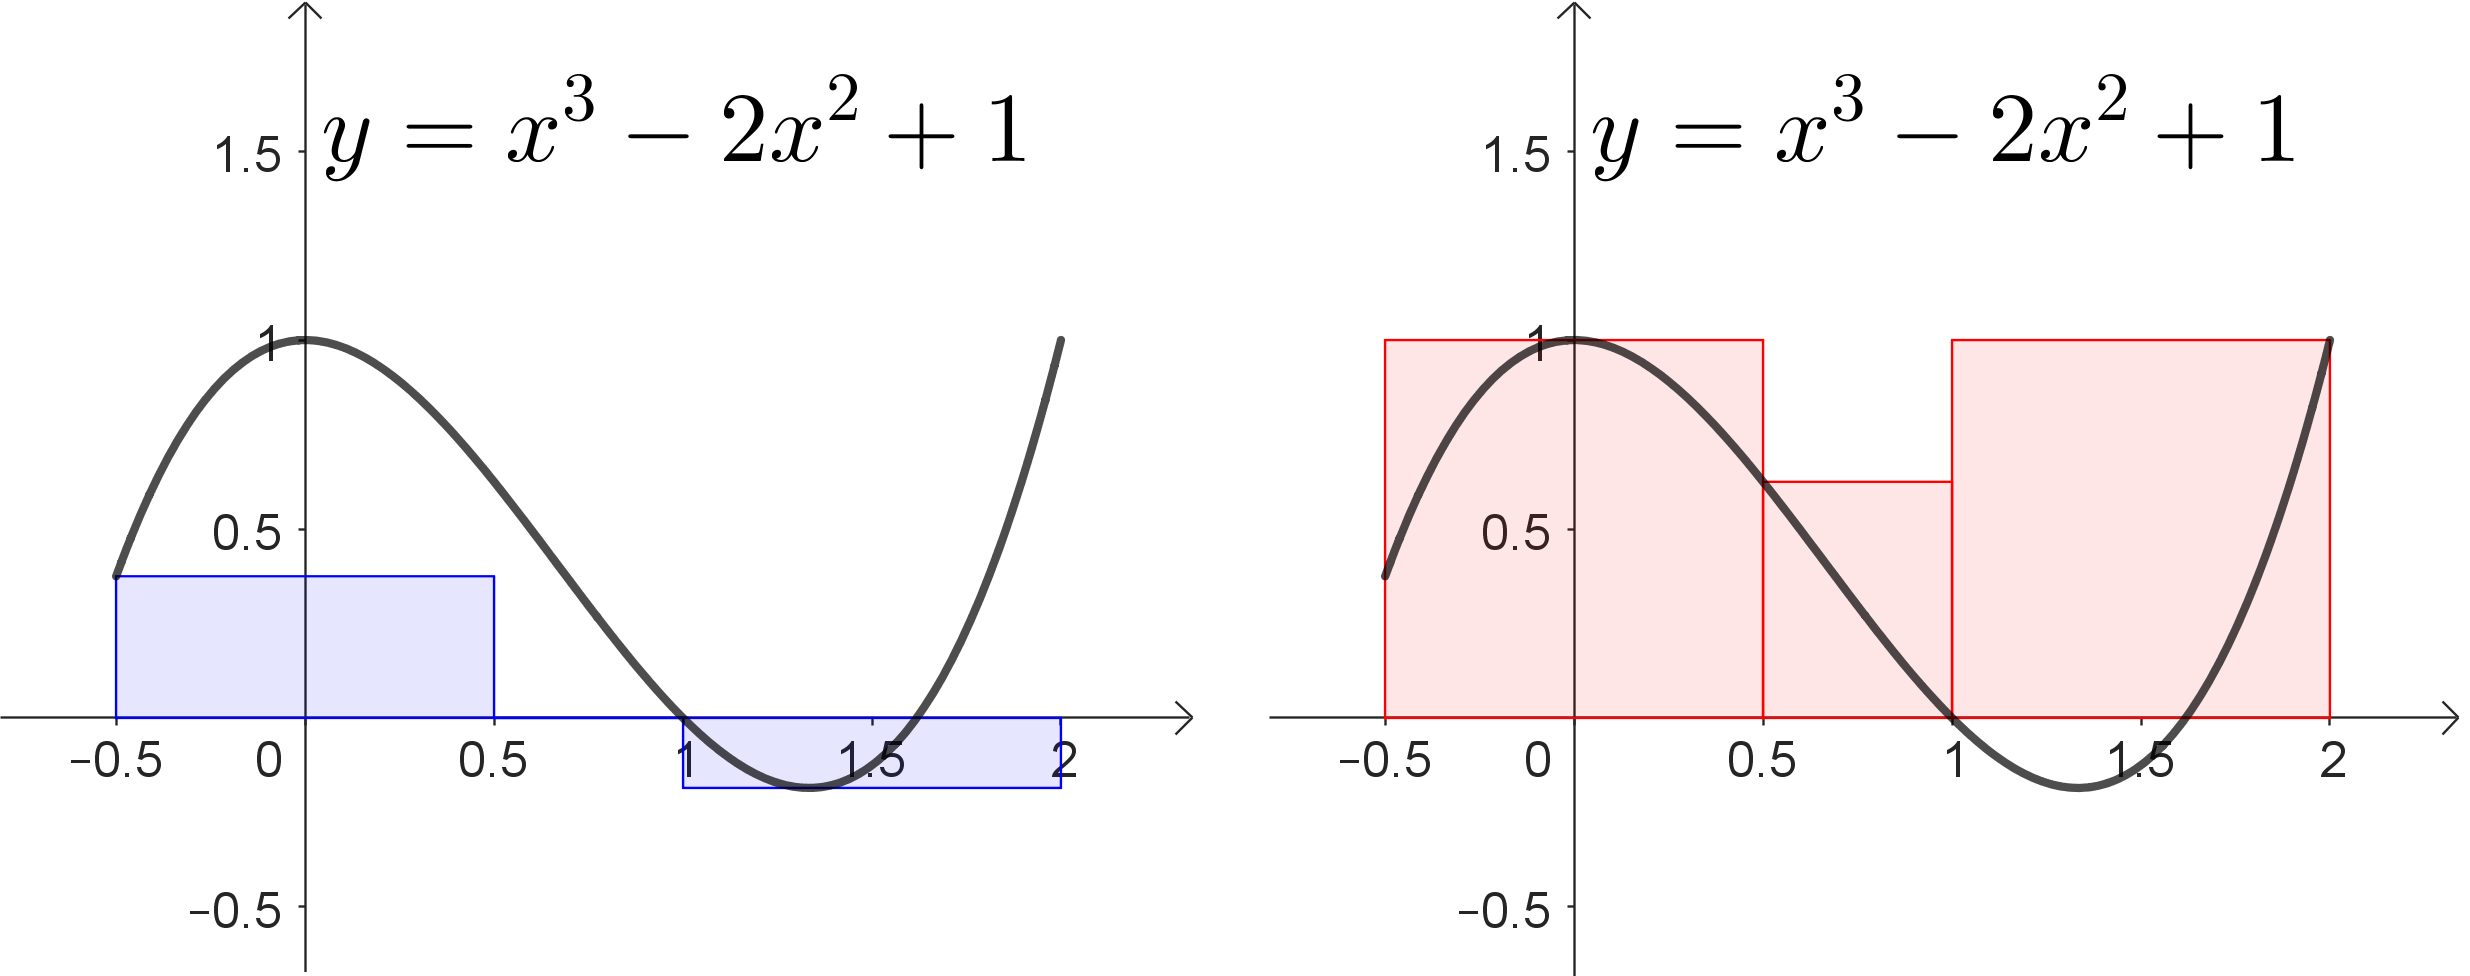
\includegraphics[width=0.95\textwidth]{Pictures/k2m9.png}
\caption{\it Myndræn framsetning á undir- og yfirsummu fallsins $f$ m.t.t skiptingarinnar $S$.}
\end{figure}

\end{syn}

\begin{hregla}{}
Gerum ráð fyrir því að $S = \{x_{0},\ldots,x_{n}\}$ sé skipting á bilinu $[a,b]$ og að $m \in [a,b]$ sé ekki í menginu $S$. Þá er $S_{m} = S \cup \{m\}$ einnig skipting á bilinu og fyrir sérhvert samfellt fall $f$ á $[a,b]$ gildir að
$$
U_{S_{m}} \geq U_{S} \; \text{ og } \; Y_{S} \geq Y_{S_{m}}
$$ 
\end{hregla}

\begin{sonnun}
Þar sem talan $m$ er ekki í menginu $S$ en á bilinu $[a,b]$ þá er þar með til tala $j$ þannig að $x_{j-1} < s < x_{j}$. Skiptingin $I_{m}$ er því eins og $I$ nema að bútnum $[x_{j-1},x_{j}]$ hefur verið skipt út en bútunum $[x_{j-1},m]$ og $[m,x_{j}]$ hefur verið skipt inn. 

\vspace{2mm}

Táknum nú lægstu gildi $f$ á bútunum $[x_{j-1},m]$ og $[m,x_{j}]$ með $l_{1}$ og $l_{2}$. Þá er ljóst að $k_{j} \leq l_{1}$ og $k_{j} \leq l_{2}$ þar sem $k_{j}$ er lægsta gildi $f$ á öllum bútnum $[x_{j-1},x_{j}]$. Skoðum nú mismuninn $U_{S_{m}} - U_{S}$. Við fáum
\begin{align*}
U_{S_{m}} - U_{S} &= \sum_{i= 1, i \neq j}^{n} k_{i}\Delta x_{i} + l_{1}\left(m-x_{j-1}\right)+l_{2}\left(x_{j} - m\right) - \sum_{i = 1}^{n} k_{i}\Delta x_{i}\\ &= l_{1}\left(m-x_{j-1}\right)+l_{2}\left(x_{j} - m\right) - k_{j}\Delta x_{j}\\ &\geq k_{j}\left(m-x_{j-1}\right)+k_{j}\left(x_{j} - m\right) - k_{j}\Delta x_{j}\\ &= k_{j}m-k_{j}x_{j-1}+k_{j}x_{j}-k_{j}m-k_{j}\Delta x_{j}\\ &= k_{j}(x_{j}-x_{j-1})-k_{j}\Delta x_{j} = k_{j}\Delta x_{j} - k_{j}\Delta x_{j} = 0
\end{align*}
Þ.e $U_{S_{m}} - U_{S} \geq 0$ og því $U_{S_{m}} \geq U_{S}$.

\vspace{2mm}

Sönnunin á ójöfnunni $Y_{S} \geq Y_{S_{m}}$ er sambærileg sönnuninni hér á undan og er eftirlátin nemendum.

\end{sonnun}

\begin{regla}{}
Ef $S$ og $T$ eru bútanir á bilinu $[a,b]$ og $T$ er fínni en $S$ þá gildir fyrir öll samfelld föll á bilinu $[a,b]$ að 
$$
U_{S} \leq U_{T} \; \text{ og } \; Y_{T} \leq Y_{S}
$$
\end{regla}

\begin{ath}
Reglan hér á undan er sönnuð með því að notast ítrekað við hjálparregluna, við eftirlátum nemendum að útfæra sönnunina.
\end{ath}

\begin{ath}
Á mannamáli segir reglan okkur að því fínni sem við gerum skiptinguna okkar, því hærra verður gildið á undirsummunni en því lægra á yfirsummunni. Því nálgast þessi gildi hvort annað þegar skiptingin er gerð fínni.
\end{ath}

\begin{regla}{}
Ef $S$ og $T$ eru bútanir á bilinu $[a,b]$ þá gildir fyrir öll samfelld föll $f$ á bilinu að
$$
U_{S} \leq Y_{T}
$$
\end{regla}

\begin{sonnun}
Athugum að $V = S \cup T$ er skipting á $[a,b]$ sem er fínni en bæði $S$ og $T$. Við fáum því 
$$
U_{S} \leq U_{V} \leq Y_{V} \leq Y_{T}
$$
\end{sonnun}

\begin{ath}
Með öðrum orðum, allar undirsummur hafa lægra gildi en allar yfirsummur.
\end{ath}

\begin{skilgr}{}
Ef $A \subseteq \mathbb{R}$ og til er tala $K$ þannig að $K \geq x$ fyrir öll $x \in A$ þá er sagt að mengið $A$ sé \textbf{takmarkað að ofan}. Eins er sagt að mengið $A$ sé \textbf{takmarkað að neðan} ef til er tala $k$ þannig að $k \leq x$ fyrir öll $x \in A$.
\end{skilgr}

\begin{frumsenda}{um fullkomleika $\mathbb{R}$}
Ef mengi $A$ er takmarkað að ofan þá er til minnsta tala $K \in \mathbb{R}$ sem uppfyllir skilyrðið $K \geq x$ fyrir öll $x \in A$. Hún er táknuð með $\sup(A)$ og nefnist \textbf{efra mark} mengisins $A$.

\vspace{2mm}

Eins gildir að ef mengið $A$ er takmarkað að neðan þá er til stærsta tala $k \in \mathbb{R}$ sem uppfyllir skilyrðið $k \leq x$ fyrir öll $x \in A$. Hún er táknuð með $\inf(A)$ og nefnist \textbf{neðra mark} mengisins $A$.

\end{frumsenda}

\begin{ath}
Í þeim tilfellum þar sem mengi $A$ hefur minnsta stak $\min(A)$ þá gildir að $\inf(A) = \min(A)$, og eins gildir að ef $A$ hefur stærsta stak $\max(A)$ þá gildir að $\sup(A) = \max(A)$. Mengi $A$ þarf þó ekki að hafa minnsta og/eða stærsta stak til þess að stærðirnar $\inf(A)$ og $\sup(A)$ séu vel skilgreindar. Ef við setjum t.d. $A = ]0,1[$ þá gildir að $\inf(A) = 0$ og $\sup(A) = 1$, en $A$ hefur hvorki minnsta né stærsta stak.
\end{ath}

\begin{skilgr}{}
Látum $f$ vera fall á bili $[a,b]$. Efra mark mengis allra undirsumma $f$ á bilinu nefnist þá \textbf{neðra heildi} fallsins $f$ yfir bilið og er táknað með $\underline{I}(f)$. Neðra mark mengis allra yfirsumma $f$ á bilinu nefnist svo \textbf{efra heildi} fallsins $f$ yfir bilið og er táknað með $\overline{I}(f)$.
\end{skilgr}

\begin{ath}
Regla $2.3$ tryggir að neðra- og efra heild falls $f$ á bili $[a,b]$ er vel skilgreint og að $\underline{I}(f) \leq \overline{I}(f)$.
\end{ath}

\begin{skilgr}{Eiginlegt heildi}
Ef um fall $f$ á bili $[a,b]$ gildir að $L = \underline{I}(f) = \overline{I}(f)$ þá er fallið sagt \textbf{heildanlegt} yfir bilið $[a,b]$. Talan $L$ kallast \textbf{eiginlega heildi} fallsins $f$ yfir bilið $[a,b]$. Við táknum eiginlega heildið með
$$
\int_{a}^{b} f(x)\;dx
$$
Tölurnar $a$ og $b$ nefnast \textbf{heildismörk} heildisins.
\end{skilgr}

\begin{ath}
Með öðrum orðum má segja að ef til er \textbf{nákvæmlega ein} tala sem er stærri en eða jöfn öllum undirsummum og minni en eða jöfn öllum yfirsummum þá er fallið $f$ heildanlegt yfir bilið $[a,b]$, en talan sem um ræðir er ákveðna heildi fallsins yfir bilið.
\end{ath}

\begin{ath}
Umfjöllun um eiginleg heildi og flatarmál.
\end{ath}

\begin{skilgr}{}
Ef $f$ er heildanlegt fall á bilinu $[a,b]$ þá skilgreinum við heildið
$$
\int_{b}^{a} f(x) \; dx = -\int_{a}^{b} f(x) \; dx
$$
\end{skilgr}

\begin{ath}
Við megum með öðrum orðum víxla á heildismörkunum í eiginlegu heildi ef við víxlum einnig formerkinu.
\end{ath}

\begin{regla}{}
Ef $f$ er heildanlegt fall á bilinu $[a,b]$ og $c \in [a,b]$ þá gildir
$$
\int_{a}^{b} f(x) \; dx = \int_{a}^{c} f(x) \; dx + \int_{c}^{b} f(x) \; dx
$$
\end{regla}

\begin{monnun}
\begin{figure}[h]
\center
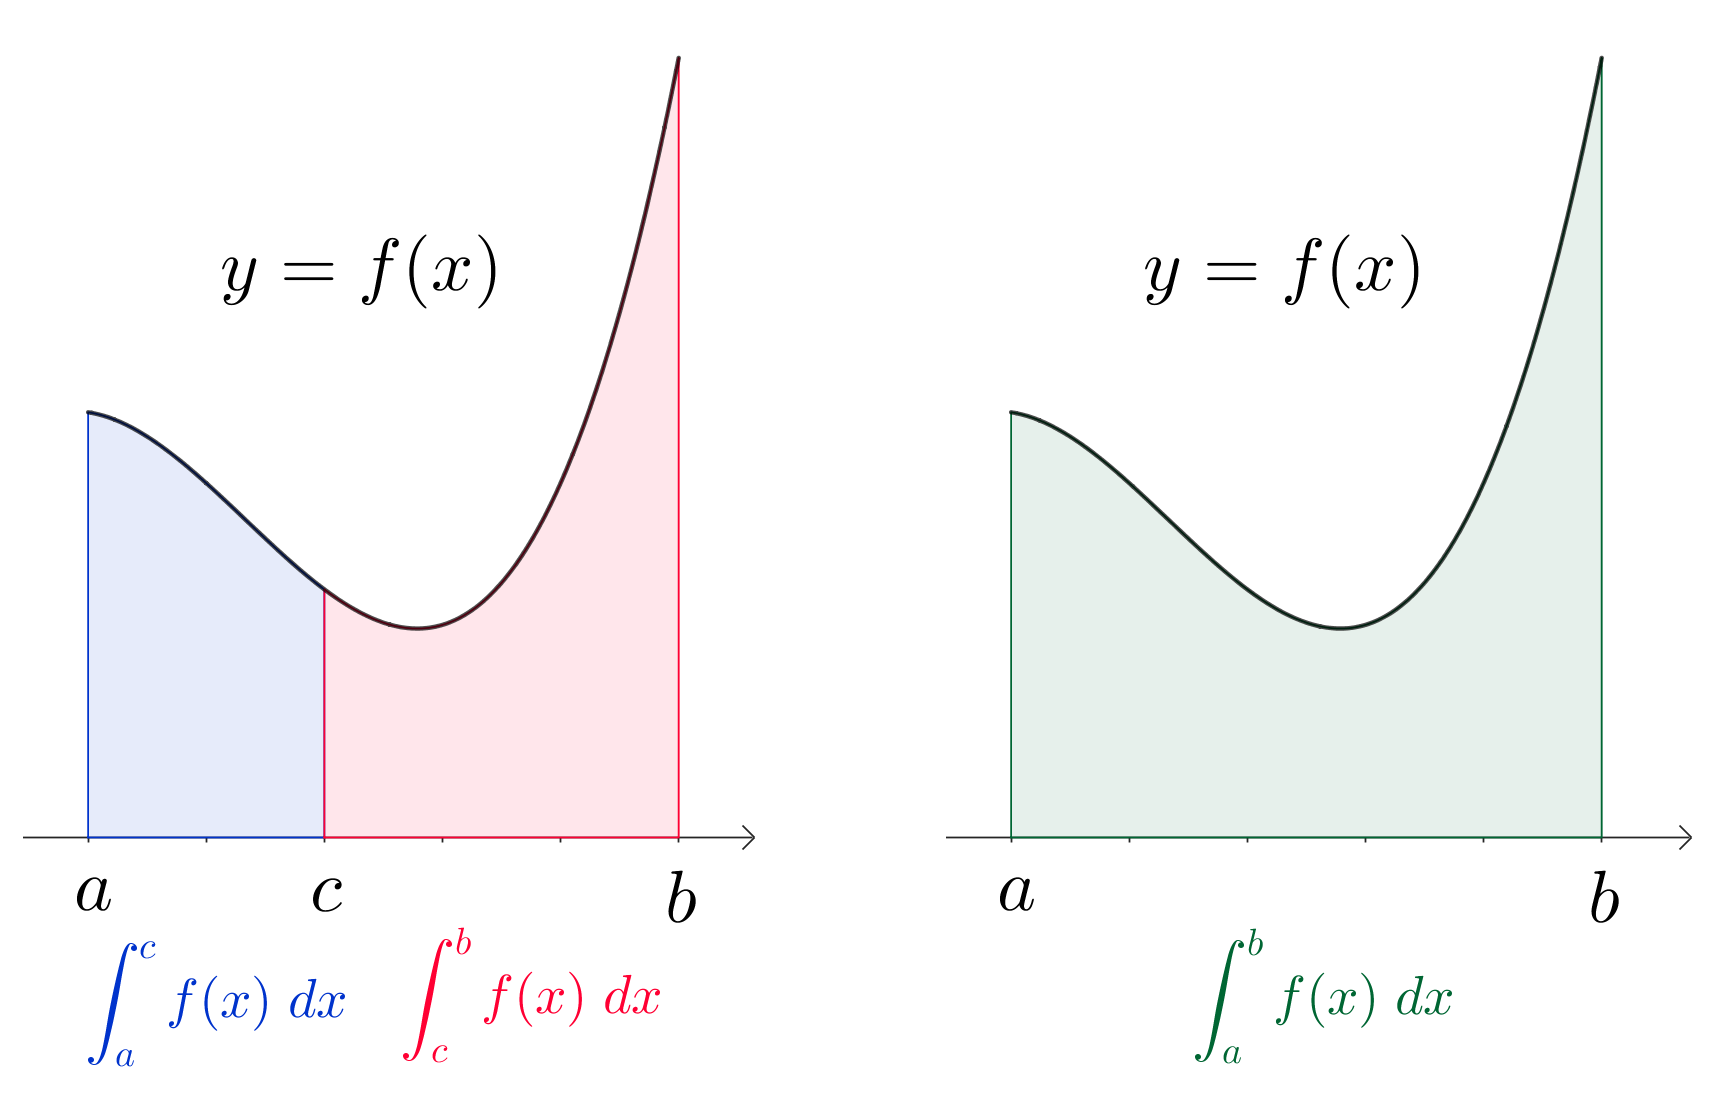
\includegraphics[width=0.8\textwidth]{Pictures/k2m5.png}
\caption{\it Myndræn framsetning á reglunni hér á undan. Samanlagt flatarmál bláa og rauða svæðisins er jafnt flatarmáli græna svæðisins.}
\end{figure}

\end{monnun}

\begin{regla}{}
Ef $f$ og $g$ eru heildanleg föll á bili $[a,b]$ og $c \in \mathbb{R}$ þá gildir:
\begin{itemize}
\item[1)] $\displaystyle \int_{a}^{b} f(x) + g(x) \; dx = \int_{a}^{b} f(x) \; dx + \int_{a}^{b} g(x) \; dx$

\item[2)] $\displaystyle \int_{a}^{b} c\cdot f(x) \; dx = c\cdot\int_{a}^{b} f(x) \; dx$
\end{itemize}
\end{regla}

\begin{regla}{}
Gerum ráð fyrir því að $S_{n}$ sé skipting á bilinu $[a,b]$ fyrir sérhvert $n \in \mathbb{N}$. Ef $f$ er fall á bilinu þannig að
$$
\lim_{n \to \infty} U_{S_{n}} = \lim_{n \to \infty} Y_{S_{n}} = L
$$
þá er fallið $f$ heildanlegt yfir bilið $[a,b]$ og
$$
\int_{a}^{b} f(x) \; dx = L
$$
\end{regla}

\begin{syn}{eiginleg heildi}
Reiknum eiginlega heildi fallsins $f(x) = x^2$ yfir bilið $[0,1]$. Notfærum okkur að $\displaystyle \sum_{k = 1}^{n} k^{2} = \frac{n(n+1)(2n+1)}{6}$.

{\bf Lausn:} Byrjum á að reikna $\displaystyle \lim_{n \to \infty} U_{I_{n}}$. Athugum að billengd sérhvers bútar í skiptingunni $I_n$ er $\frac{1-0}{n} = \frac{1}{n}$ og að fallið $f$ er vaxandi svo lægsta gildi þess er tekið í vinstri endapunkti sérhvers bútar. Við sjáum einnig að $x_{k} = \frac{k}{n}$ og því fæst:
\setlength{\jot}{4mm}
\begin{align*}
U_{I_{n}} &= \sum_{k = 1}^{n} x_{k-1}^{2}\cdot\Delta x_{k}\\ &= \sum_{k = 1}^{n} \left(\frac{k-1}{n}\right)^{2}\cdot\frac{1}{n}\\ &= \frac{1}{n^{3}}\cdot\sum_{k = 0}^{n-1} k^{2} = \frac{1}{n^{3}}\cdot\sum_{k = 1}^{n-1} k^{2}\\ &= \frac{1}{n^{3}} \cdot \frac{(n-1)n(2n-1)}{6}\\ &= \frac{2n^{3}-3n^{2}+n}{6n^{3}} = \frac{1}{3}-\frac{1}{2n}+\frac{1}{6n^{2}}
\end{align*}
Þar með fæst að $\displaystyle \lim_{n \to \infty} U_{I_{n}} = \frac{1}{3}$.

\vspace{2mm}

Þegar yfirsumman m.t.t. $I_{n}$ er reiknuð þá notfærum við okkur að hæsta fallgildi $f$ á hverjum bút er tekið í hægri endapunkta bútarins og fáum með sambærilegum hætti og hér að ofan að
$$
Y_{I_{n}} = \sum_{k = 1}^{n}x_{k}^{2}\Delta x_{k} = \frac{2n^{3}+3n^{2}+n}{6n^{3}} = \frac{1}{3}+\frac{1}{2n}+\frac{1}{6n^{2}}
$$
og þar með $\displaystyle \lim_{n \to \infty} Y_{I_{n}} = \frac{1}{3}$.

\vspace{2mm}

Við fáum því að
$$
\int_{0}^{1} x^{2}\;dx = \frac{1}{3}
$$

\end{syn}

\begin{regla}{Meðalgildisreglan fyrir heildi}
Ef $f$ er samfellt fall á bili $[a,b]$ þá er til tala $c \in [a,b]$ þannig að
$$
f(c) = \frac{1}{b-a}\int_{a}^{b} f(x) \; dx
$$
\end{regla}

\begin{sonnun}
Setjum $S = \{a,b\}$. Þá er $S$ skipting á bilinu $[a,b]$ og því gildir að
$$
U_{S} \leq \int_{a}^{b} f(x) \; dx \leq Y_{S}
$$
Ef við látum nú $k$ vera lággildi $f$ á $[a,b]$ en $K$ hágildi þess á bilinu þá höfum við þar með
$$
k(b-a) \leq \int_{a}^{b} f(x) \; dx \leq K(b-a)
$$
og því
$$
k \leq \frac{1}{b-a}\int_{a}^{b} f(x) \; dx \leq K
$$
Milligildisreglan fyrir samfelld föll gefur því að til er $c \in [a,b]$ þannig að
$$
f(c) = \frac{1}{b-a}\int_{a}^{b} f(x) \; dx
$$

\begin{figure}[H]
\center
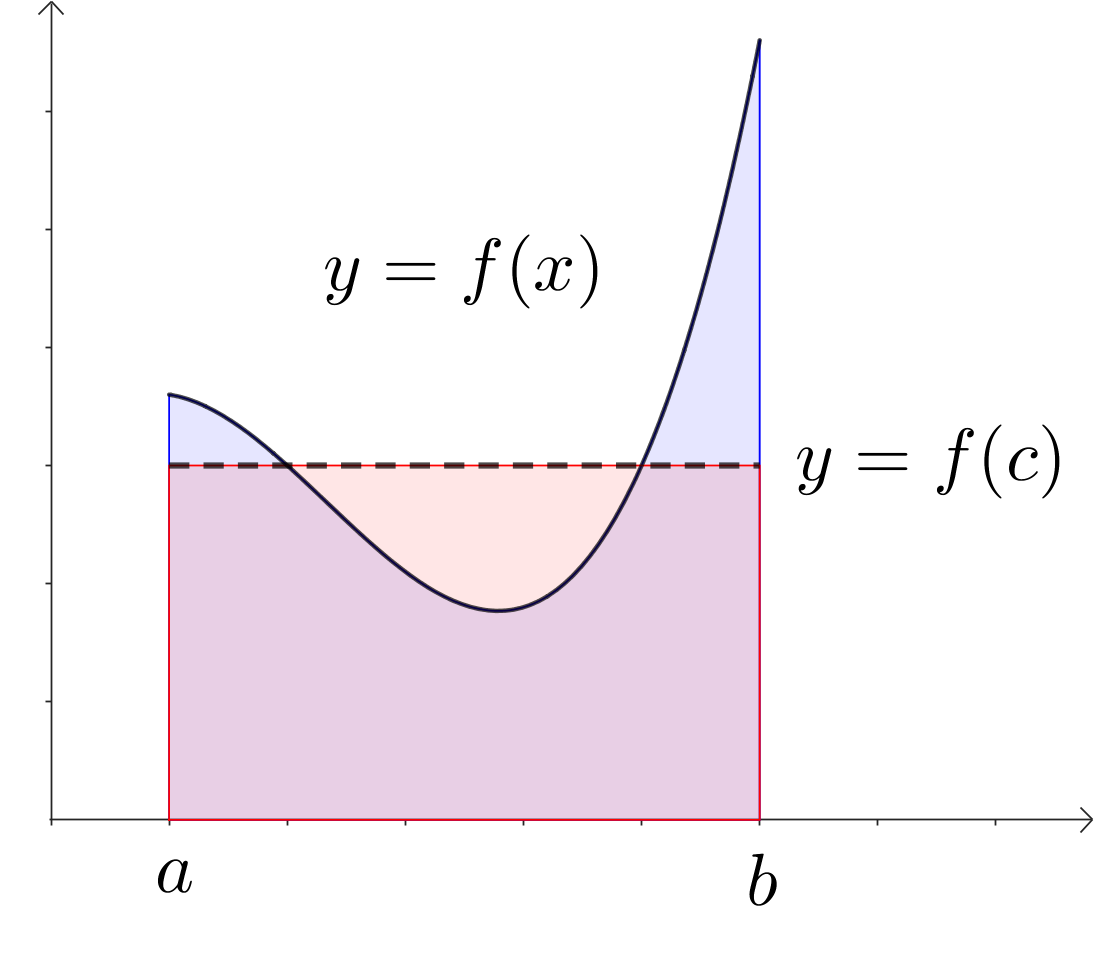
\includegraphics[width=0.8\textwidth]{Pictures/k2m10.png}
\caption{\it Myndræn framsetning á meðalgildisreglunni fyrir heildi. Flatarmálið undir ferli fallsins $f$ á bilinu $[a,b]$ er jafnt $\displaystyle \int_{a}^{b} f(x)\;dx = f(c)(b-a)$}
\end{figure}

\end{sonnun}

\begin{regla}{Undirstöðusetning stærðfræðigreiningarinnar} 
Ef $f$ er samfellt fall á $[a,b]$ og við skilgreinum fyrir öll $x \in [a,b]$ fallið
$$
F(x) = \int_{a}^{x} f(t)\;dt
$$
þá gildir að $F'(x) = f(x)$.
\end{regla}

\begin{sonnun}
Byrjum á að skoða afleiðuna frá hægri, fáum:
\begin{align*}
F'_{+}(x) &= \lim_{h \to 0^{+}} \dfrac{F(x+h)-F(x)}{h}\\ &= \lim_{h \to 0^{+}} \dfrac{\int_{a}^{x+h}f(t)\;dt - \int_{a}^{x}f(t)\;dt}{h}\\ &= \lim_{h \to 0^{+}} \dfrac{\int_{x}^{x+h}f(t)\;dt}{h}\\ &= \lim_{h \to 0^{+}} \frac{1}{h}\int_{x}^{x+h}f(t)\;dt
\end{align*}

Athugum nú að lengd bilsins $[x,x+h]$ er $h$, og því gefur meðalgildisreglan fyrir heildi að fyrir sérhvert $h>0$ er til tala $c_{h}$ á bilinu $[x,x+h]$ þannig að
$$
f\left(c_{h}\right) = \frac{1}{h}\int_{x}^{x+h}f(t)\;dt
$$

Þegar $h$ stefnir á $0$ þá hlítur svo talan $c_{h}$ að vera að stefna á $x$ þar sem hún er klemmd á milli $x$ og $x+h$. Samfelldni fallsins $f$ gefur því:

\begin{align*}
F'_{+}(x) = \lim_{h \to 0^{+}} f\left(c_{h}\right) = f(x) 
\end{align*}

Tilfellið fyrir vinstri afleiðuna er sambærilegt, við þurfum einungis að athuga að í því tilfelli er talan $c_h$ á bilinu $[x+h,x]$ og við þurfum að huga örlítið að formerkjum í útreikningum okkar. Nemendum er eftirlátið að fylla í eyðurnar.
\end{sonnun}

\begin{ath}
Í reglunni hér að ofan túlkum við $F'(a)$ sem afleiðu fallsins $F$ frá hægri, en $F'(b)$ sem afleiðu fallsins $F$ frá vinstri.
\end{ath}

\begin{regla}{Undirstöðusetning stærðfræðigreiningarinnar - 2. útgáfa}
Ef $f$ er samfellt fall á $[a,b]$ og $F$ er stofnfall fyrir $f$ þá gildir
$$
\int_{a}^{b}f(x)\;dx = F(b) - F(a)
$$
\end{regla}

\begin{sonnun}
Ef við skilgreinum $G(t) = \int_{a}^{t}f(x)\;dx$ þá er $G$ stofnfall fyrir $f$ skv. meginsetningu stærðfræðigreiningarinnar. Ef $F$ er eitthvert annað stofnfall fyrir $G$ þá gildir svo að til er fasti $k$ þannig að
$$
F(t) = G(t) + k
$$
Þar sem $G(a) = 0$ þá fæst þar með að $F(a) = k$ og því fáum við 
$$
G(t) = F(t) - k = F(t) - F(a)
$$
Setjum $t = b$ og fáum svo
$$
\int_{a}^{b} f(x)\;dx = G(b) = F(b)-F(a)
$$
\end{sonnun}

\begin{ath}
Mjög algengt er að notast við ritháttinn $\displaystyle \Biggl[F(x)\Biggr]_{a}^{b}$ fyrir $F(b) - F(a)$. Við getum þá skrifað regluna hér á undan sem
$$
\int_{a}^{b}f(x)\;dx = \Biggl[F(x)\Biggr]_{a}^{b} = F(b) - F(a)
$$
\end{ath}

\begin{syn}{ákveðin heildi}
Reiknum eftirfarandi ákveðnu heildi:
\begin{itemize}
\item[1)] $\displaystyle \int_{1}^{2} 2x^{2}-x+1 \; dx$

\item[2)] $\displaystyle \int_{4}^{5} \frac{2}{x-3} \; dx$

\item[3)] $\displaystyle \int_{0}^{1} 5\cos(\pi x) \; dx$
\end{itemize}

\vspace{2mm}

{\bf Lausn:}
\begin{itemize}
\item[1)]
\begin{align*}
\int_{1}^{2} 3x^{2}-x+1 \; dx = \Biggl[x^{3}-\frac{1}{2}x^{2}+x\Biggr]_{1}^{2} = 2^{3}-\frac{1}{2} \cdot 2^{2}+2 - \left(1^{3}-\frac{1}{2} \cdot 1 + 1\right) = 6.5
\end{align*}
\item[2)]
\begin{align*}
\int_{4}^{5} \frac{2}{x-3} \; dx = 2\cdot\Biggl[\ln(x-3)\Biggr]_{4}^{5} = 2\cdot\left(\ln(5)-\ln(4)\right) = 2\ln\left(\frac{5}{4}\right) = 0.446
\end{align*}
\item[3)]
\begin{align*}
\int_{0}^{1} 5\cos(\pi x) \; dx = 5\cdot\Biggl[\frac{1}{\pi}\sin(\pi x)\Biggr]_{0}^{1} = \frac{5}{\pi}\cdot\left(\sin(\pi)-\sin(0)\right) = 0
\end{align*}
\end{itemize}
\end{syn}

\begin{æd}
Reiknið eftirfarandi ákveðnu heildi:
\begin{itemize}
\item[1)] $\displaystyle \int_{1}^{3} -x^{2}+x+3 \; dx$

\item[2)] $\displaystyle \int_{0}^{1} 3^{x} \; dx$

\item[3)] $\displaystyle \int_{\pi}^{2\pi} 2\sin(x) \; dx$
\end{itemize}
\end{æd}

\begin{regla}{Hlutheildun - Ákveðin heildi}
Ef $f$ er heildanlegt fall á bili $[a,b]$ og $g$ diffranlegt á sama bili þá gildir að
$$
\int_{a}^{b} f(x)g'(x) \; dx = \Biggl[f(x)g(x)\Biggr]_{a}^{b} - \int_{a}^{b} f'(x)g(x)\;dx
$$
\end{regla}

\begin{syn}{hlutheildun}
Reiknum eftirfarandi heildi með því að notast við hlutheildun.
\begin{itemize}
\item[1)] $\displaystyle \int_{0}^{1} xe^{x} \; dx$

\item[2)] $\displaystyle \int_{0}^{\pi} x\sin(x) \; dx$

\item[3)] $\displaystyle \int_{1}^{e} 2x^{2}\ln(x) \; dx$
\end{itemize}

\vspace{2mm}

{\bf Lausn:}
\begin{itemize}
\item[1)] Við veljum $f(x) = x$ og $g'(x) = e^{x}$. Þá er $f'(x) = 1$ og $g(x) = e^{x}$ og við fáum því:
\setlength{\jot}{4mm}
\begin{align*}
\int_{0}^{1} xe^{x}\;dx &= \Biggl[xe^{x}\Biggr]_{0}^{1}-\int_{0}^{1}e^{x}\;dx = 1\cdot e^{1}-0\cdot e^{0} - \Biggl[e^{x}\Biggr]_{0}^{1}\\ &= e - \left(e^{1}-e^{0}\right) = e^{0} = 1
\end{align*}

\item[2)] Veljum $f(x) = x$ og $g'(x) = \sin(x)$. Þá er $f'(x) = 1$ og $g(x) = -\cos(x)$ svo við fáum:
\begin{align*}
\int_{0}^{\pi} x\sin(x) \; dx &= \Biggl[-x\cos(x)\Biggr]_{0}^{\pi} + \int_{0}^{\pi} \cos(x) \; dx = -\pi\cos(\pi)-(-0\cdot\cos(0)) + \Biggl[\sin(x)\Biggr]_{0}^{\pi}\\ &= \pi + (\sin(\pi)-\sin(0)) = \pi
\end{align*}

\item[3)] Veljum $f(x) = \ln(x)$ og $g'(x) = 2x^{2}$. Þá er $f'(x) = \frac{1}{x}$ og $g(x) = \frac{2}{3}x^{3}$. Því fæst:
\begin{align*}
\int_{1}^{e} 2x^{2}\ln(x) \; dx &= \Biggl[\frac{2}{3}x^{3}\ln(x)\Biggr]_{1}^{e} - \int_{1}^{e} \frac{2}{3}x^{2} \; dx = \frac{2}{3}e^{3}\ln(e)-\frac{2}{3}e^{1}\ln(1) - \Biggl[\frac{2}{9}x^{3}\Biggr]_{1}^{e}\\ &= \frac{2}{3}e^{3}-\left(\frac{2}{9}e^{3}-\frac{2}{9}\cdot 1^{3}\right) = \frac{2}{9}\left(2e^{3}+1\right)
\end{align*}
\end{itemize}

\end{syn}

\begin{æd}
Reiknið eftirfarandi heildi með því að notast við hlutheildun.
\begin{itemize}
\item[1)] $\displaystyle \int_{0}^{2} x2^{x} \; dx$

\item[2)] $\displaystyle \int_{0}^{\pi} x\cos(2x) \; dx$

\item[3)] $\displaystyle \int_{1}^{2} \sqrt{x}\ln(x) \; dx$
\end{itemize}
\end{æd}

\begin{regla}{Innsetningarregla - Ákveðin heildi}
Tökum föll $f$ og $g$ og bil $[a,b]$ þannig að $f\circ g$ sé heildanlegt á $g\left([a,b]\right)$ og $g$ diffranlegt. Ef $u = g(x)$ þá er $du = g'(x)\;dx$ og
$$
\int_{a}^{b} f(g(x))\cdot g'(x)\;dx = \int_{g(a)}^{g(b)} f(u)\;du
$$
\end{regla}

\begin{syn}{innsetningu}
Reiknum eftirfarandi heildi með því að notast við innsetningu.
\begin{itemize}
\item[1)] $\displaystyle \int_{-1}^{1} 3x^{2}\left(x^{3}+1\right)^{5} \; dx$

\item[2)] $\displaystyle \int_{e}^{e^{2}} \frac{\ln(\ln(x))}{x}  \; dx$

\item[3)] $\displaystyle \int_{0}^{\frac{\pi}{2}} \cos(x)\sin^{2}(x) \; dx$
\end{itemize}

\vspace{2mm}

{\bf Lausn:}
\begin{itemize}
\item[1)] Setjum $u = x^{3}+1$. þá er $du = 3x^{2} \; dx$. Athugum einnig að ef $x = -1$ þá höfum við $u = 0$ og ef $x = 1$ þá fæst $u = 2$. Við fáum því
$$
\int_{-1}^{1} 3x^{2}\left(x^{3}+1\right)^{5} \; dx = \int_{0}^{2} u^{5} \; du = \Biggl[\frac{1}{6}u^{6}\Biggr]_{0}^{2} = \frac{32}{3}
$$

\item[2)] Setjum nú $u = \ln(x)$. Þá er $du = \frac{1}{x}\; dx$. Einnig höfum við að ef $x = e$ þá er $u = 1$ og ef $x = e^{2}$ þá er $u = 2$. Því fæst
\setlength{\jot}{4mm}
\begin{align*}
\int_{e}^{e^{2}} \frac{\ln(\ln(x))}{x}  \; dx &= \int_{1}^{2} \ln(u) \; du = \Biggl[u\ln(u)-u\Biggr]_{1}^{2}\\ &= 2\ln(2)-2-\left(1\cdot\ln(1)-1\right)\\ &= \ln(4)-1 = 0.386
\end{align*}

\item[3)] Hér setjum við $u = \sin(x)$. Þá höfum við að $du = \cos(x) \; dx$. Einnig höfum við að þegar $x = 0$ þá er $u = 0$ og þegar $x = \frac{\pi}{2}$ þá er $u = 1$. Við fáum því
$$
\int_{0}^{\frac{\pi}{2}} \cos(x)\sin^{2}(x) \; dx = \int_{0}^{1} u^{2} \; du = \Biggl[\frac{1}{3}u^{3}\Biggr]_{0}^{1} = \frac{1}{3}
$$
\end{itemize}
\end{syn}

\begin{æd}
Reiknið eftirfarandi heildi með því að notast við innsetningu.
\begin{itemize}
\item[1)] $\displaystyle \int_{1}^{3} 4x\sqrt{x^{2+1}} \; dx$

\item[2)] $\displaystyle \int_{0}^{1} x^{2}e^{x^{3}} \; dx$

\item[3)] $\displaystyle \int_{1}^{2} \frac{2\ln(x)}{x}\; dx$
\end{itemize}
\end{æd}

% Setja þessa niðurstöðu fram í dæmakafla
%%%%%%%%%%%%%%%
\begin{comment}
\begin{regla}{}
Ef $f$ og $g$ eru heildanleg föll á bili $[-a,a]$ með $a \geq 0$, $f$ er oddstætt og $g$ er jafnstætt þá gildir:
\begin{itemize}
\item[1)] $\displaystyle \int_{-a}^{a} f(x) \; dx = 0$

\item[2)] $\displaystyle \int_{-a}^{a} g(x) \; dx = 2\int_{0}^{a} g(x) \; dx$
\end{itemize}

\end{regla}

\begin{sonnun}
\begin{itemize}
\item[1)] Þar sem $f$ er oddstætt þá gildir þar með $f(-x) = -f(x)$ fyrir öll $x \in [-a,a]$. Við fáum því:
\begin{align*}
\int_{-a}^{a} f(x) \; dx = \underbrace{\int_{-a}^{0} f(x) \; dx}_{\text{Setjum } u = -x} + \int_{0}^{a} f(x) \; dx = 
\end{align*}
\end{itemize}
\end{sonnun}
\end{comment}
%%%%%%%%%%%%%%%%

\if \kafli1
{\newpage}
\fi

\label{sec:ÆfingEiginlegheildi}
\subsubsection*{Æfing \ref{sec:ÆfingEiginlegheildi}}
\begin{adjustwidth}{-\hangingaefingar}{}
\begin{enumerate}

\item Reiknið undir-, yfir- og millisummur eftirfarandi falla.
\begin{enumerate}
\setlength\itemsep{4mm}
\item $f(x) = 2x$ á bilinu $[0,2]$ m.t.t. skiptingarinnar $S = \left\{0,\frac{1}{2},\frac{3}{2},2\right\}$

\item $h(x) = \frac{1}{x^{2}}$ á bilinu $[0,3]$ m.t.t. jöfnu skiptingarinnar $I_{3}$.

\item $g(x) = e^{x}$ á bilinu $[0,1]$ m.t.t. skiptingarinnar $S = \left\{0,\frac{1}{2},\frac{5}{6},1\right\}$. Skilið svarinu með $3$ aukastöfum.

\item $f(x) = \cos(x)$ á bilinu $\left[0,\pi\right]$ m.t.t. skiptingarinnar $S = \left\{0,\frac{\pi}{4},\frac{\pi}{2},\pi\right\}$. Skilið svarinu með $3$ aukastöfum.
\end{enumerate}

\vspace{2mm}

\item Finnið útgildi fallsins $f$ á bilinu $[a,b]$ og gerið formerkjamynd fyrir afleiðuna. Notið svo niðurstöðurnar til þess að finna undir- og yfirsummu fallsins $f$ m.t.t. skiptingarinnar $S$.

\begin{enumerate}
\setlength\itemsep{4mm}

\item $f(x) = \frac{1}{2}x^{3}-x$, $[a,b] = \left[-1,2\right]$ og $S = \left\{-1,0,\frac{3}{2},2\right\}$.

\item $f(x) = $, $[a,b] = $ og $S = \left\{\right\}$.
\end{enumerate}

\vspace{2mm}

\item Notist við gröf eftirfarandi falla til þess að reikna heildin.
\begin{enumerate}
\item Eitthvað
\end{enumerate}

\vspace{2mm}

\item Reiknið eftirfarandi heildi.
\begin{multicols}{2}
\begin{enumerate}
\setlength\itemsep{4mm}
\item $\displaystyle \int_{}^{} \; dx$
\item $\displaystyle \int_{}^{} \; dx$
\item $\displaystyle \int_{}^{} \; dx$
\item $\displaystyle \int_{}^{} \; dx$
\item $\displaystyle \int_{}^{} \; dx$
\item $\displaystyle \int_{}^{} \; dx$
\item $\displaystyle \int_{}^{} \; dx$
\item $\displaystyle \int_{}^{} \; dx$
\item $\displaystyle \int_{}^{} \; dx$
\item $\displaystyle \int_{}^{} \; dx$
\item $\displaystyle \int_{}^{} \; dx$
\item $\displaystyle \int_{}^{} \; dx$
\item $\displaystyle \int_{}^{} \; dx$
\item $\displaystyle \int_{}^{} \; dx$
\item $\displaystyle \int_{}^{} \; dx$
\item $\displaystyle \int_{}^{} \; dx$
\end{enumerate}
\end{multicols}

\vspace{2mm}

\item Gefið er fallið $f(x) = x$ á bilinu $[0,1]$. Sýnið að $\displaystyle \lim_{n \to \infty} U_{I_{n}} = \lim_{n \to \infty} Y_{I_{n}}$ og notfærið ykkur svo þessa niðurstöðu til þess að ákvarða $\displaystyle \int_{0}^{1} f(x) \; dx$.

\vspace{2mm}

\item Gefin eru föll $f$ og $g$ á bilinu $[-a,a]$ með $a > 0$. Einnig er vitað að $f$ er \textbf{oddstætt fall} en $g$ er \textbf{jafnstætt}. Sýnið að þá gildi eftirfarandi reglur:
\begin{enumerate}
\setlength\itemsep{4mm}
\item $\displaystyle \int_{-a}^{a} f(x) \; dx = 0$
\item $\displaystyle \int_{-a}^{a} g(x) \; dx = 2\int_{0}^{a} g(x) \; dx$
\end{enumerate}

\vspace{2mm}

\item Skilgreinum fallið $\ln : ]0,\infty[ \to \mathbb{R}$ með því að setja
$$
\ln(x) = \int_{1}^{x} \frac{1}{t} \; dt
$$
Notist við skilgreininguna til þess að sýna eftirfarandi:
\begin{enumerate}
\setlength\itemsep{4mm}
\item $\displaystyle \left(\ln(x)\right)' = \frac{1}{x}$
\item $\displaystyle \ln\left(a^{b}\right) = b\ln(a)$
\item $\displaystyle \ln\left(ab\right) = \ln(a)+\ln(b)$
\item $\displaystyle \ln\left(\frac{a}{b}\right) = \ln(a) - \ln(b)$
\end{enumerate}

\vspace{2mm}

\item Sýna að fallið $\displaystyle f(x) = \begin{cases} 1 \text{ ef x er óræð tala}\\ 0 \text{ ef x er ræð tala}\end{cases}$ sé ekki heildanlegt á $[0,1]$. Sýna fyrst að milli sérhverra talna sé til ræð og óræð tala.

\end{enumerate}
\end{adjustwidth}

\fi

\if \kafli1
{\if \svor1 \newpage \fi}
\fi


\if \svor1
\textbf{Svör við æfingu \ref{sec:ÆfingEiginlegheildi}}
\begin{enumerate}

\item %Segið til um hvort eftirfarandi föll séu hlutleysuföll, fastaföll, veldisföll, margliður og/eða ræð föll.
\begin{multicols}{2}
\begin{enumerate}
\item Fastafall og 0. stigs margliða %$f:\mathbb{R}\rightarrow\mathbb{R}$ með $f(x)=-2$
\item Veldisfall og 2. stigs margliða %$g:\mathbb{R}\rightarrow\mathbb{R}$ með $g(x)=x^2$
\item Hlutleysufall og 1. stigs margliða %$h:\mathbb{R}\rightarrow\mathbb{R}$ með $h(x)=x$
\item 1. stigs margliða %$i:\mathbb{R}\rightarrow\mathbb{R}$ með $i(x)=x+1$
\item Veldisfall $\left(x^{\frac{1}{2}}\right)$ %$j:\mathbb{R_+}\rightarrow\mathbb{R}$ með $j(x)=\sqrt{x}$
\item Fastafall og margliða sem hefur ekkert stig %$k:\mathbb{R}\rightarrow\mathbb{R}$ með $k(x)=0$
\item Rætt fall %$l:\mathbb{R_+}\rightarrow\mathbb{R}$ með $l(x)=\frac{x-2}{x+2}$
\item 3. stigs margliða %$m:\mathbb{R}\rightarrow\mathbb{R}$ með $m(x)=x^3+x^2$
\end{enumerate}
\end{multicols}

\item %Teiknið ferla þessara falla í höndum.
\begin{multicols}{2}
\begin{enumerate}
\item %$f(x)=x^3$
\begin{tikzpicture}[mynd, x=1cm, y=0.2cm, baseline=(Y.base)]
\draw[asar] (-2.5,0) -- (2.5,0) node [xas] {$x$};
\foreach \x in {-2,-1,1,2}
\draw[xkvardi, shift={(\x,0)}] (0pt,2pt) -- (0pt,-2pt) node[xkvardi] {$\x$};
\draw[asar] (0,-15) -- (0,15) node [yas] (Y) {$y$};
\foreach \y in {-10,-5,5,10}
\draw[ykvardi, shift={(0,\y)}] (2pt,0pt) -- (-2pt,0pt) node[ykvardi] {$\y$};
\draw[ferill,domain=-2.4:2.4] plot(\x,{\x^3});
\end{tikzpicture}

\item %$g(x)=\sqrt{x}$
\begin{tikzpicture}[mynd, x=1cm, y=1cm, baseline=(Y.base)]
\draw[asar] (-1,0) -- (4,0) node [xas] {$x$};
\foreach \x in {1,2,3}
\draw[xkvardi, shift={(\x,0)}] (0pt,2pt) -- (0pt,-2pt) node[xkvardi] {$\x$};
\draw[asar] (0,-0.5) -- (0,2.5) node [yas] (Y) {$y$};
\foreach \y in {1,2}
\draw[ykvardi, shift={(0,\y)}] (2pt,0pt) -- (-2pt,0pt) node[ykvardi] {$\y$};
\draw[ferill,domain=0:3.5] plot(\x,{sqrt(\x)});
\end{tikzpicture}

\end{enumerate}
\end{multicols}

\item Svari sleppt.

\end{enumerate}
\fi

